\documentclass[a4paper,11pt]{book}
%\documentclass[a4paper,twoside,11pt,titlepage]{book}
\usepackage{listings}
\usepackage[utf8]{inputenc}
\usepackage[spanish]{babel}

% \usepackage[style=list, number=none]{glossary} %
%\usepackage{titlesec}
%\usepackage{pailatino}

\decimalpoint
\usepackage{dcolumn}
\newcolumntype{.}{D{.}{\esperiod}{-1}}
\makeatletter
\addto\shorthandsspanish{\let\esperiod\es@period@code}
\makeatother


%\usepackage[chapter]{algorithm}
\RequirePackage{verbatim}
%\RequirePackage[Glenn]{fncychap}
\usepackage{fancyhdr}
\usepackage{graphicx}
\usepackage{afterpage}

\usepackage{longtable}

\usepackage[pdfborder={000}]{hyperref} %referencia

% ********************************************************************
% Re-usable information
% ********************************************************************
\newcommand{\myTitle}{Título del proyecto\xspace}
\newcommand{\myDegree}{Grado en ...\xspace}
\newcommand{\myName}{Nombre Apllido1 Apellido2 (alumno)\xspace}
\newcommand{\myProf}{Nombre Apllido1 Apellido2 (tutor1)\xspace}
\newcommand{\myOtherProf}{Nombre Apllido1 Apellido2 (tutor2)\xspace}
%\newcommand{\mySupervisor}{Put name here\xspace}
\newcommand{\myFaculty}{Escuela Técnica Superior de Ingenierías Informática y de
Telecomunicación\xspace}
\newcommand{\myFacultyShort}{E.T.S. de Ingenierías Informática y de
Telecomunicación\xspace}
\newcommand{\myDepartment}{Departamento de ...\xspace}
\newcommand{\myUni}{\protect{Universidad de Granada}\xspace}
\newcommand{\myLocation}{Granada\xspace}
\newcommand{\myTime}{\today\xspace}
\newcommand{\myVersion}{Version 0.1\xspace}


\hypersetup{
pdfauthor = {\myName (email (en) ugr (punto) es)},
pdftitle = {\myTitle},
pdfsubject = {},
pdfkeywords = {palabra_clave1, palabra_clave2, palabra_clave3, ...},
pdfcreator = {LaTeX con el paquete ....},
pdfproducer = {pdflatex}
}

%\hyphenation{}


%\usepackage{doxygen/doxygen}
%\usepackage{pdfpages}
\usepackage{url}
\usepackage{colortbl,longtable}
\usepackage[stable]{footmisc}
\usepackage{eurosym}
\usepackage{float}
\usepackage{listings}
\usepackage{color}
\usepackage{graphicx}
\usepackage{caption}
\usepackage{subcaption}
%\usepackage{index}

%\makeindex
%\usepackage[style=long, cols=2,border=plain,toc=true,number=none]{glossary}
% \makeglossary

% Definición de comandos que me son tiles:
%\renewcommand{\indexname}{Índice alfabético}
%\renewcommand{\glossaryname}{Glosario}

\pagestyle{fancy}
\fancyhf{}
\fancyhead[LO]{\leftmark}
\fancyhead[RE]{\rightmark}
\fancyhead[RO,LE]{\textbf{\thepage}}
\renewcommand{\chaptermark}[1]{\markboth{\textbf{#1}}{}}
\renewcommand{\sectionmark}[1]{\markright{\textbf{\thesection. #1}}}

\setlength{\headheight}{1.5\headheight}

\newcommand{\HRule}{\rule{\linewidth}{0.5mm}}
%Definimos los tipos teorema, ejemplo y definición podremos usar estos tipos
%simplemente poniendo \begin{teorema} \end{teorema} ...
\newtheorem{teorema}{Teorema}[chapter]
\newtheorem{ejemplo}{Ejemplo}[chapter]
\newtheorem{definicion}{Definición}[chapter]

\definecolor{gray97}{rgb}{1,1,1}
\definecolor{gray45}{rgb}{0.5,0.5,0.5}
\definecolor{gray}{rgb}{0.9,0.9,0.9}
\definecolor{dkgreen}{rgb}{0,0.6,0}
\definecolor{mauve}{rgb}{0.58,0,0.82}
\definecolor{verde}{rgb}{0.55,0.71,0.0}
\definecolor{azuloscuro}{rgb}{0.0,0.44,1.0}
\definecolor{naranja}{rgb}{0.91,0.45,0.32}
\definecolor{amarillo}{rgb}{0.94,0.86,0.51}
\definecolor{morado}{rgb}{0.0,0.2,0.4}
\definecolor{violeta}{rgb}{0.45,0.31,0.59}
\definecolor{verdelima}{rgb}{0.5,1.0,0.0}
\definecolor{rojo}{rgb}{0.89,0.26,0.2}
\definecolor{gris}{rgb}{0.5,0.5,0.5}
\definecolor{rosa}{rgb}{1.0,0.33,0.5}


\lstset{
	language=python,
	aboveskip=3mm,
	belowskip=3mm,
	showstringspaces=false,
	columns=flexible,
	basicstyle={\small\ttfamily},
	numbers=none,
	numberstyle=\tiny\color{gray},
	keywordstyle=\color{blue},
	commentstyle=\color{dkgreen},
	stringstyle=\color{mauve},
	breaklines=true,
	breakatwhitespace=false,
	tabsize=3
}

\lstset{ frame=Ltb,
     framerule=0.5pt,
     aboveskip=0.5cm,
     framextopmargin=3pt,
     framexbottommargin=3pt,
     framexleftmargin=0.1cm,
     framesep=0pt,
     rulesep=.4pt,
     backgroundcolor=\color{gray97},
     rulesepcolor=\color{black},
     %
     stringstyle=\ttfamily,
     showstringspaces = false,
     basicstyle=\scriptsize\ttfamily,
     commentstyle=\color{gray45},
     keywordstyle=\bfseries,
     %
     numbers=left,
     numbersep=6pt,
     numberstyle=\tiny,
     numberfirstline = false,
     breaklines=true,
   }
   
  
 
% minimizar fragmentado de listados
\lstnewenvironment{listing}[1][]
   {\lstset{#1}\pagebreak[0]}{\pagebreak[0]}

\lstdefinestyle{CodigoC}
   {
	basicstyle=\scriptsize,
	frame=single,
	language=C,
	numbers=left
   }
\lstdefinestyle{CodigoC++}
   {
	basicstyle=\small,
	frame=single,
	backgroundcolor=\color{gray30},
	language=C++,
	numbers=left
   }
 
\lstdefinestyle{Consola}
   {basicstyle=\scriptsize\bf\ttfamily,
    backgroundcolor=\color{gray30},
    frame=single,
    numbers=none
   }


\newcommand{\bigrule}{\titlerule[0.5mm]}


%Para conseguir que en las páginas en blanco no ponga cabecerass
\makeatletter
\def\clearpage{%
  \ifvmode
    \ifnum \@dbltopnum =\m@ne
      \ifdim \pagetotal <\topskip
        \hbox{}
      \fi
    \fi
  \fi
  \newpage
  \thispagestyle{empty}
  \write\m@ne{}
  \vbox{}
  \penalty -\@Mi
}
\makeatother

\usepackage{pdfpages}
\begin{document}
\begin{titlepage}
 
 
\newlength{\centeroffset}
\setlength{\centeroffset}{-0.5\oddsidemargin}
\addtolength{\centeroffset}{0.5\evensidemargin}
\thispagestyle{empty}

\noindent\hspace*{\centeroffset}\begin{minipage}{\textwidth}

\centering

\includegraphics[width=0.9\textwidth]{imagenes/logo_ugr.jpg}\\[1.4cm]

\textsc{ \Large TRABAJO FIN DE GRADO\\[0.2cm]}
\textsc{ Grado en Ingeniería Informática}\\[1cm]
% Upper part of the page
% 
% Title
{\Huge\bfseries drawercloud\\
}
\noindent\rule[-1ex]{\textwidth}{3pt}\\[3.5ex]
{\large\bfseries Aplicación web orientada al almacenamiento de archivos en la nube}
\end{minipage}

\vspace{2.5cm}
\noindent\hspace*{\centeroffset}\begin{minipage}{\textwidth}
\centering

\textbf{Autor}\\ {José Manuel Rejón Santiago (alumno)}\\[2.5ex]
\textbf{Director}\\
{Prof. Dr. José María Guirao Miras (tutor)}\\[2cm]

\includegraphics[width=0.3\textwidth]{imagenes/etsiit_logo.png}\\[0.1cm]
\textsc{Escuela Técnica Superior de Ingenierías Informática y de Telecomunicación}\\
\textsc{---}\\
Granada, Septiembre de 2017
\end{minipage}
%\addtolength{\textwidth}{\centeroffset}
%\vspace{\stretch{2}}
\end{titlepage}



\chapter*{}
%\thispagestyle{empty}
%\cleardoublepage

%\thispagestyle{empty}

\begin{titlepage}
 
 
\setlength{\centeroffset}{-0.5\oddsidemargin}
\addtolength{\centeroffset}{0.5\evensidemargin}
\thispagestyle{empty}

\noindent\hspace*{\centeroffset}\begin{minipage}{\textwidth}

\centering
%
\includegraphics[width=0.9\textwidth]{imagenes/logo_ugr.jpg}\\[1.4cm]

%\textsc{ \Large PROYECTO FIN DE CARRERA\\[0.2cm]}
%\textsc{ INGENIERÍA EN INFORMÁTICA}\\[1cm]
% Upper part of the page
% 

 \vspace{3.3cm}

%si el proyecto tiene logo poner aquí

\includegraphics[width=1\textwidth]{imagenes/logo.png} 
 \vspace{0.5cm}

% Title

{\Huge\bfseries drawercloud\\
}
\noindent\rule[-1ex]{\textwidth}{3pt}\\[3.5ex]
{\large\bfseries Aplicación web orientada al almacenamiento de archivos en la nube.\\[4cm]}
\end{minipage}

\vspace{2.5cm}
\noindent\hspace*{\centeroffset}\begin{minipage}{\textwidth}
\centering

\textbf{Autor}\\ {José Manuel Rejón Santiago (alumno)}\\[2.5ex]
\textbf{Director}\\
{Prof. Dr. José María Guirao Miras}\\[2cm]
%
\includegraphics[width=0.15\textwidth]{imagenes/tstc.png}\\[0.1cm]
%\textsc{Departamento de Teoría de la Señal, Telemática y Comunicaciones}\\
%\textsc{---}\\
%Granada, mes de 201
\end{minipage}
%\addtolength{\textwidth}{\centeroffset}
\vspace{\stretch{2}}

 
\end{titlepage}




\clearpage
\thispagestyle{empty}

\begin{center}
{\large\bfseries drawercloud: aplicación web orientada al almacenamiento de archivos en la nube}\\
\end{center}
\begin{center}
José Manuel Rejón Santiago (alumno)\\
\end{center}

%\vspace{0.7cm}
\noindent{\textbf{Palabras clave}: aplicación web, cloud, pc, tablet, smartphone, servidor web, framework, responsive design}\\

\vspace{0.5cm}
\noindent{\textbf{Resumen}}\\

\textbf{drawercloud} es una aplicación web para el alojamiento de archivos en la nube (cloud). Los usuarios podrán realizar diversas tareas sobre sus archivos, como por ejemplo: Añadir/Eliminar archivos en la nube, reproducir archivos multimedia, organizar archivos en directorios, compartir archivos, descargar en un dispositivo (pc, tablet, smartphone)... De este modo, conseguiremos tener nuestros archivos almacenados en un servidor web, ahorrando espacio en nuestros dispositivos y con la seguridad de tener nuestro material a salvo en otro lugar.\\

Para el desarrollo de la web usaremos \textbf{Django} \cite{cita1}, que es un framework para aplicaciones web gratuito y open source, escrito en \textbf{Python} \cite{cita2}. La aplicación web contará con un \textbf{responsive design} para ser adaptada a otros dispositivos (como smartphones o tablets). En el lado del servidor, se usará la tecnología proporcionada por Amazon Web Services o Google.\\

Para el aspecto gráfico usamos la tecnología que nos ofrece \textbf{Twitter Bootstrap} \cite{cita3}, un framework \textbf{HTML} \cite{cita4}, \textbf{CSS} \cite{cita5} y \textbf{JavaScript} \cite{cita6} para lograr un diseño web adaptable (responsive design) entre los distintos dispositivos que puedan hacer uso de la aplicación web. \textbf{Ajax} \cite{cita7} y \textbf{jQuery} \cite{cita8} serán las herramientas elegidas para ofrecer una mejor interacción entre el usuario y la aplicación web. \\

La base de datos será gestionada con \textbf{MongoDB} \cite{cita9}, que es una base de datos orientada a documentos estilo JSON (incluye información del tipo de dato). \\

drawercloud hace uso de \textbf{EC2} \cite{cita_ec2} (Amazon Virtual Servers), que nos permite alojar la web gratuitamente durante un año y poder acceder a ella desde cualquier dispositivo que se conecte a la red. Como servidor web usamos \textbf{NGINX} \cite{cita_nginx} y \textbf{Gunicorn} \cite{cita_gunicorn} que es un WSGI de Python.\\

Este proyecto está bajo la licencia de software libre, lo que significa que los usuarios tienen la libertad de ejecutar, copiar, distribuir, estudiar, modificar y mejorar el software.

\clearpage


\thispagestyle{empty}


\begin{center}
{\large\bfseries drawercloud: aplicación web orientada al almacenamiento de archivos en la nube}\\
\end{center}
\begin{center}
José Manuel Rejón Santiago (student)\\
\end{center}

%\vspace{0.7cm}
\noindent{\textbf{Keywords}: Keyword1, Keyword2, Keyword3, ....}\\

\vspace{0.7cm}
\noindent{\textbf{Abstract}}\\

Write here the abstract in English.

\chapter*{}
\thispagestyle{empty}

\noindent\rule[-1ex]{\textwidth}{2pt}\\[4.5ex]

Yo, \textbf{José Manuel Rejón Santiago}, alumno de la titulación Grado en Ingeniería Informática de la \textbf{Escuela Técnica Superior
de Ingenierías Informática y de Telecomunicación de la Universidad de Granada}, con DNI 20077299R, autorizo la
ubicación de la siguiente copia de mi Trabajo Fin de Grado en la biblioteca del centro para que pueda ser
consultada por las personas que lo deseen.

\vspace{6cm}

\noindent Fdo: José Manuel Rejón Santiago

\vspace{2cm}

\begin{flushright}
Granada a 12 de Septiembre de 2017.
\end{flushright}


\chapter*{}
\thispagestyle{empty}

\noindent\rule[-1ex]{\textwidth}{2pt}\\[4.5ex]

D. \textbf{Prof. Dr. José María Guirao Miras (tutor)}, Profesor del Departamento de Lenguajes y Sistemas Informáticos de la Universidad de Granada.

\vspace{0.5cm}

\textbf{Informan:}

\vspace{0.5cm}

Que el presente trabajo, titulado \textit{\textbf{drawercloud, aplicación web orientada al almacenamiento de archivos en la nube}},
ha sido realizado bajo su supervisión por \textbf{José Manuel Rejón Santiago (alumno)}, y autoriza la defensa de dicho trabajo ante el tribunal
que corresponda.

\vspace{0.5cm}

Y para que conste, expiden y firman el presente informe en Granada a 12 de Septiembre de 2017.

\vspace{1cm}

\textbf{El tutor:}

\vspace{5cm}

\noindent \textbf{Prof. Dr. José María Guirao Miras}

\chapter*{Agradecimientos}
\thispagestyle{empty}

       \vspace{1cm}


En primer lugar quiero mostrar mi agradecimiento a mi tutor José María Guirao Miras por darme la oportunidad de realizar este proyecto y toda la ayuda y consejos recibidos. \\

También agradecer a mi familia y amigos/as que han estado apoyándome durante todo el desarrollo del proyecto como a lo largo de estos años de carrera. \\

Por último y no menos importante a mis compañeros durante esta experiencia, un gran apoyo siempre tanto dentro como fuera de clase.




%\frontmatter
\tableofcontents
\listoffigures
\listoftables
%
%\mainmatter
%\setlength{\parskip}{5pt}

\chapter{Introducción}

El objetivo de este proyecto es el desarrollo de una aplicación web que proporcione al usuario la posibilidad de almacenar sus archivos en la nube. La aplicación web cuenta con opciones como el almacenamiento en un lugar seguro, la organización por carpetas, la posibilidad de crear grupos de trabajo donde compartir los archivos con compañeros, entre otras más.

\section{Motivación}

Unos de los problemas que surgen en el uso de nuestros dispositivos es el almacenamiento. Es cierto que el precio del \textbf{gigabyte} es cada vez más barato e incluso más rápido (como por ejemplo en los discos duros SSD, que están dotados de un gran incremento de velocidad, además de consumir menos energía) pero, aunque en un ordenador el almacenamiento puede no ser un problema, si que lo es si hablamos de dispositivos móviles como smartphones o tablets. A día de hoy, encontramos dispositivos que no permiten la insercción de tarjetas de almacenamiento flash, lo cual nos obliga a conformarnos con el espacio que el fabricante pone a nuestra disposición (o a comprar el modelo con más capacidad, pero obviamente más caro). \textbf{drawercloud} viene a poner solución a este problema, ofreciendo un espacio personal en un servidor web dedicado para dicha aplicación, de modo que nuestros datos permanecen en tal servidor sin ocupar memoria en nuestros dispositivos. \\

¿Significa esto que solo es una solución para dispositivos que cuentan con un espacio muy limitado? No, ya que otro problema que puede surgirnos con mucha facilidad es la pérdida de información por diversas causas (disco duro roto, pérdida del dispositivo, virus, etc) y para ello este proyecto también ofrece una solución a dicho problema. Podemos almacenar nuestros archivos tanto en el disco duro propio del dispositivo en cuestión, como en el espacio ofrecido en el servidor web, de modo que si nos vemos afectados por alguno de los motivos mencionados, o bien por otros que afectan a la desaparición de nuestra información, tengamos una copia en otro lugar y no perdamos nuestros archivos. \\

Otro caso en el que esta aplicación resulta interesante es que podemos disponer de nuestros datos en cualquier parte. A modo de ejemplo, podemos pensar en un archivo que estamos modificando en casa y en nuestro puesto de trabajo. Almacenando dicho archivo en la nube nos tenemos que olvidar de mover la información a través de, por ejemplo, un pen drive o de tener una copia en casa y otra en la oficina y andar actualizando ambas cada vez que queramos trabajar. Simplemente entraremos con nuestra cuenta a \textbf{drawercloud} desde cualquier dispositivo y tendremos acceso al archivo en cuestión. Además, proporciona un método para compartir archivos y crear grupos de trabajo, de modo que si sobre ese archivo están trabajando, por ejemplo, 3 personas más, podrán ver las modificaciones que hemos realizado directamente sobre el archivo alojado en el servidor web.

\chapter{Análisis}

\section{Estudio de mercado}
Antes de comenzar el desarrollo del proyecto es recomendable realizar un estudio de mercado. Dicho estudio nos ofrecerá una visión de las virtudes y carencias de los productos que actualmente ofrecen un servicio similar y así, saber en que punto nos encontraremos respecto a ellos. Ésto nos dará la ventaja de poder realzar los puntos fuertes de nuestro proyecto frente a la competencia. Veamos algunos ejemplos de aplicaciones que ofrecen el mismo servicio: \\

\subsection{Dropbox \cite{cita_dropbox}}
Dropbox es la aplicación para almacenar archivos en la nube posiblemente más conocida y usada, siendo ésta una de las primeras en ofrecernos este tipo de servicios. En su versión gratuita, los usuarios de esta aplicación disponen de 2GB, pero se puede ampliar hasta 16GB realizando algunas sencillas tareas (como subir fotos desde el móvil o recomendar a amigos). Por 9,99 \euro/mes se dispondrá de 1TB de espacio disponible. \textbf{Equipo} y \textbf{Paper} son dos opciones que ofrece Dropbox para trabajar en equipo, siendo éstas dos puntos fuertes de este servicio. También su aplicación de escritorio es un punto muy a favor, dando la posibilidad al usuario de sincronizar sus datos más rápidamente (aunque puede ralentizar el arranque del pc mientras sincroniza). \\

\subsection{Google Drive \cite{cita_google_drive}}
Como era de esperar, no podía faltar Google en esta lista. En su versión gratuita ofrece 15GB de almacenamiento (sin necesidad de realizar tareas para ampliar como hace dropbox). Para ampliar el espacio, Google Drive ofrece dos posibilidades:
\begin{enumerate}
	\item 100GB por 1,99 \euro/mes
	\item 1TB por 9,99 \euro/mes
\end{enumerate}
Sin duda, el punto fuerte de Google Drive es la posibilidad de crear archivos (como hojas de texto, hojas de cálculo, formularios, ...) que pueden ser editados por otras personas (si le damos el permiso de compartir) y así trabajar en grupo sobre el mismo documento en la nube, almacenando los cambios automáticamente. \\


\subsection{Mega \cite{cita_mega}}
Aunque es más conocido por la piratería, Mega es otra de las solucines para alojar archivos en la nube. Ofrece hasta 50GB de forma de gratuita y en caso de querer más espacio, se pueden usar estas alternativas:
\begin{enumerate}
	\item 500GB por 9,99 \euro/mes
	\item 2TB por 19,99 \euro/mes
	\item 4TB por 29,99 \euro/mes
\end{enumerate}
Además de la enorme cantidad de espacio, el alto ancho de banda que ofrece sería un punto a favor de Mega. \\

\subsection{OneDrive \cite{cita_onedrive}}
OneDrive es la solución para almacenamiento en la nube propuesta por Microsoft. Viene preinstalado en Windows 10 y eso permite que los documentos y las fotografías se guarden automáticamente en OneDrive. Ofrece también un apartado de empresas para que un grupo de trabajo pueda colaborar sobre los mismos archivos en tiempo real (permite colaborar con Word, Excel, PowerPoint, OneNote).
La versión gratuita de este servicio se ha reducido a 5GB (siendo antes 15GB). Las soluciones de pago son las siguientes:
\begin{enumerate}
	\item 50GB por 2,00 \euro/mes
	\item 1TB por 7,00 \euro/mes (incluye Office 365 y la opción de instalar en un PC o Mac y en una tablet y un smartphone)
	\item 5TB (1000 GB por usuario) por 10,00 \euro/mes (incluye Office 365 y la opción de instalar en 5 PC o Mac y en 5 tablets y 5 smartphones)
\end{enumerate}

\section{Objetivos del sistema}
El objetivo principal del sistema es poner a disposición del usuario un espacio de almacenamiento en la nube. En dicho espacio, el usuario tendrá la posibilidad de almacenar información de forma organizada, compartir los archivos deseados y tener accesibilidad a éstos desde cualquier plataforma con un navegador web. \\

Con el fin de ofrecer un sistema fiable a los clientes, este programa deberá cumplir algunas características:
\begin{itemize}
	\item Disponibilidad: los datos del usuario siempre estarán disponibles.
	\item Seguridad: los datos deberán estar alojados en un lugar protegido de posibles amenazas.
	\item Accesibilidad: los datos del usuario siempre estarán disponibles para él y para quien tenga permisos sobre ellos.
\end{itemize}

Visto el objetivo principal, se listan los objetivos específicos a realizar para la realización de esta aplicación web:
\begin{itemize}
	\item \textbf{OBJ-1:} El sistema deberá almacenar los archivos relativos a cada usuario en su espacio disponible.
	\item \textbf{OBJ-2:} El sistema deberá permitir el acceso a la información solo a los usuarios con los permisos necesarios.
	\item \textbf{OBJ-3:} El sistema deberá ser accesible desde todos los dispositivos dotados de navegador web (ordenador, smartphone, tablet, etc).
\end{itemize}

\section{Requisitos funcionales del sistema}
En esta sección indicamos qué debe hacer el sistema:

\begin{itemize}
	\item \textbf{RF-1: Gestión de usuarios.} En el sistema realizaremos altas, bajas y modificaciones de los usuarios.
	\begin{itemize}
		\item \textbf{RF-1.1: Alta usuario.} El sistema permite realizar el alta de un usuario.
		\item \textbf{RF-1.2: Baja usuario.} El sistema permite realizar la baja de un usuario.
		\item \textbf{RF-1.3: Modificación usuario.} El sistema permite realizar una modificación de un usuario.
		\item \textbf{RF-1.4: Consulta usuario.} El sistema permite realizar una consulta de un usuario en concreto.
	\end{itemize}
	
	\item \textbf{RF-2: Gestión de archivos.}
	\begin{itemize}
		\item \textbf{RF-2.1: Añadir archivo.} Junto al archivo se añadirá una serie de datos como nombre, fecha de subida, propietario, etc.
		\item \textbf{RF-2.2: Eliminar archivo.} Se eliminará el archivo y toda la información relativa a él.
		\item \textbf{RF-2.3: Visualizar archivo.} Se podrá ver el contenido del archivo que sea posible (como reproducir canciones o ver una imagen).
		\item \textbf{RF-2.4: Descargar archivo.} Descarga el archivo en el dispositivo usado.
		\item \textbf{RF-2.5: Compartir archivo.} Da acceso al archivo (en modo lectura) a otro usuario.
		\item \textbf{RF-2.6: Dejar de compartir archivo.} Retira el acceso al archivo a otro usuario.
		\item \textbf{RF-2.7: Cambiar nombre del archivo.} Permite cambiar el nombre del archivo.
		\item \textbf{RF-2.8: Copiar archivo.} Se creará una copia del archivo.
		\item \textbf{RF-2.9: Mover archivo.} Se moverá el archivo al directorio de destino seleccionado.
		\item \textbf{RF-2.10: Añadir archivo a favoritos.} El archivo pasará a la lista de favoritos.
		\item \textbf{RF-2.10: Eliminar archivo de favoritos.} El archivo dejará la lista de favoritos.
		\item \textbf{RF-2.11: Añadir archivo a mi nube.} El archivo compartido (en modo lectura) pasará a ser un archivo propiedad del usuario.
	\end{itemize}
	
	\item \textbf{RF-3: Gestión de directorios.}
	\begin{itemize}
		\item \textbf{RF-3.1: Añadir directorio.} Junto al directorio se añadirá una serie de datos como nombre, contenido, propietario y directorio padre.
		\item \textbf{RF-3.2: Eliminar directorio.} Se eliminará el directorio y todos los directorios y archivos que contenga.
		\item \textbf{RF-3.3: Visualizar directorio.} Acceder al contenido del directorio.
		\item \textbf{RF-3.4: Cambiar nombre directorio.} Permite cambiar el nombre del directorio.
		\item \textbf{RF-3.5: Copiar directorio.} Se creará una copia del directorio y todo su contenido.
		\item \textbf{RF-3.6: Mover directorio.} Se moverá el directorio y todo su contenido al directorio de destino seleccionado.
	\end{itemize}
	
	\item \textbf{RF-4: Gestión de grupos de trabajo.}
	\begin{itemize}
		\item \textbf{RF-4.1: Añadir grupo de trabajo.} Se añade un grupo con un nombre.
		\item \textbf{RF-4.2: Ver grupo de trabajo.} Visualiza el contenido del grupo de trabajo.
		\item \textbf{RF-4.3: Salir del grupo de trabajo.} Un usuario sale del grupo de trabajo. Cuando el grupo de trabajo queda sin usuarios, se elimina toda la información relativa a él.
		\item \textbf{RF-4.4: Añadir participante al grupo de trabajo.} Se añade un participante al grupo con todos los permisos (subir archivo, eliminar archivo, crear carpeta, añadir participante, etc).
		\item \textbf{RF-4.5: Ver participantes del grupo de trabajo.} Se muestran todos los participantes del grupo.
	\end{itemize}
\end{itemize}

\section{Requisitos no funcionales del sistema}
En esta sección se incluyen restricciones que afectarán a los requisitos funcionales:

\begin{itemize}
	\item \textbf{RNF-1: Seguridad de la información.} Ante un posible fallo del sistema, la información previamente almacenada no debería perderse. En principio esto se garantiza, ya que el sistema y la base de datos son entidades relacionadas pero separadas. Sería buena práctica tener en cuenta la posibilidad de realizar copias de seguridad periódicamente o alguna otra alternativa que permita replicar los datos.
	\item \textbf{RNF-2: Concurrencia.} Tanto administradores como usuarios podrán acceder simultáneamente al sistema, introducciendo información, consultándola o eliminándola.
	\item \textbf{RNF-3: Autenticación.} Es necesario controlar el acceso de los usuarios, de manera que cada uno pueda realizar sólo las tareas sobre su espacio.
	\item \textbf{RNF-4: Legales.} Se deben tener en cuenta ciertos criterios de responsabilidad sobre los datos publicados, como que los datos de un usuario no sean accesibles por otro.
	\item \textbf{RNF-5: Rendimiento.} El sistema debe tener un tiempo de respuesta	y aprovechamiento de los recursos óptimo.
\end{itemize}

\section{Requisitos de información}
En esta sección se indica la información que es necesaria almacenar en el sistema:

\begin{itemize}
	\item \textbf{RI-1: Usuarios.} Datos sobre las personas que usarán la aplicación.
	\begin{itemize}
		\item \textbf{Contenido:} nombre de usuario, contraseña, dirección de correo electrónico.
		\item \textbf{Requisitos asociados:} RF-1, RNF-1, RNF-3.
	\end{itemize}
	
	\item \textbf{RI-2: Archivos.} Datos sobre los archivos que se alojarán en la aplicación.
	\begin{itemize}
		\item \textbf{Contenido:} archivo, nombre del archivo, tipo del archivo, fecha de subida, propietario, tamaño del archivo, booleano para indicar si es favorito.
		\item \textbf{Requisitos asociados:} RF-2, RNF-1, RNF-3, RNF-4, RNF-5.
	\end{itemize}
	
	\item \textbf{RI-3: Directorios.} Datos sobre los directorios que se alojarán en la aplicación.
	\begin{itemize}
		\item \textbf{Contenido:} nombre del directorio, cotenido del directorio, propietario.
		\item \textbf{Requisitos asociados:} RF-3, RNF-1, RNF-3, RNF-4, RNF-5.
	\end{itemize}
	
	\item \textbf{RI-4: Grupos de trabajo.} Datos sobre los grupos de trabajo de la aplicación.
	\begin{itemize}
		\item \textbf{Contenido:} nombre del grupo de trabajo, usuarios que pertenecen al grupo de trabajo, directorios que pertenecen al grupo de trabajo, archivos que pertenecen al grupo de trabajo.
		\item \textbf{Requisitos asociados:} RF-4, RNF-1, RNF-4, RNF-5.
	\end{itemize}
\end{itemize}

\section{Casos de uso}
\subsection{Descripción de los actores}
\begin{itemize}
	\item \textbf{DA-1: Usuario.}
	\begin{itemize}
		\item \textbf{Descripción:} Usuario que accede al sistema para gestionar su espacio personal o sus grupos de trabajo.
		\item \textbf{Características:} Conocimientos básicos sobre el manejo de algún dispositivo con navegador web.
		\item \textbf{Relaciones:} La relación con otros usuarios del sistema se da, o bien compartiendo un archivo directamente con el usuario, o bien perteneciendo al mismo grupo de trabajo.
		\item \textbf{Referencias:} Puede consultar la base de datos de sus archivos, directorios, grupos de trabajo, información asociada a su perfil y la ayuda.
	\end{itemize}
\end{itemize}
\subsection{Diagramas del modelo de casos de uso}
Los diagramas de casos de uso representan como el usuario se relaciona con el sistema para usar sus funciones. A continuación vemos dichos diagramas:

\begin{figure}[H]
	\centering
	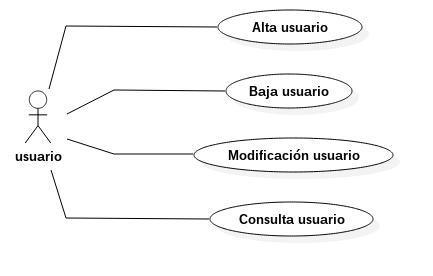
\includegraphics[width=0.7\textwidth]{imagenes/casouso_usuario}
	\caption{Diagrama de casos de uso. Gestión de usuarios.}
	\label{fig:casouso_usuario}
\end{figure}

\begin{figure}[H]
	\centering
	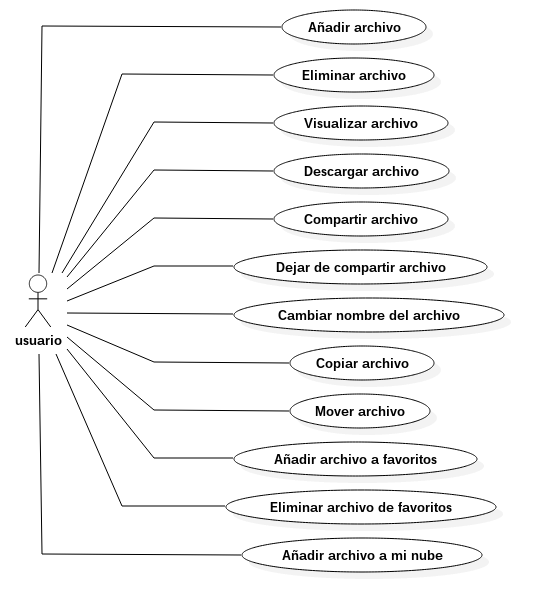
\includegraphics[width=0.7\textwidth]{imagenes/casouso_archivo}
	\caption{Diagrama de casos de uso. Gestión de archivos.}
	\label{fig:casouso_archivo}
\end{figure}

\begin{figure}[H]
	\centering
	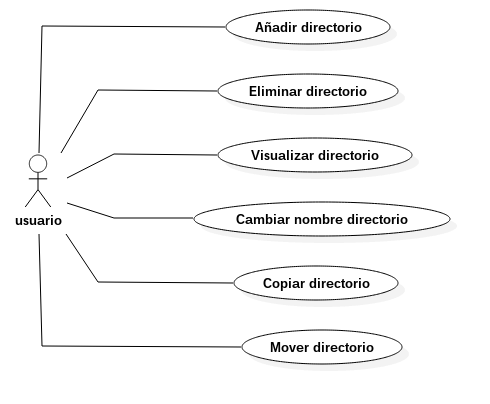
\includegraphics[width=0.7\textwidth]{imagenes/casouso_directorio}
	\caption{Diagrama de casos de uso. Gestión de archivos.}
	\label{fig:casouso_directorio}
\end{figure}

\begin{figure}[H]
	\centering
	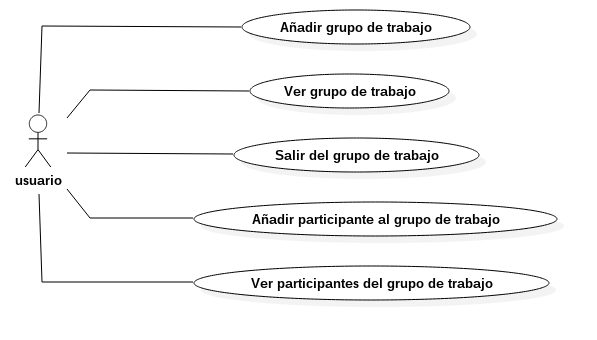
\includegraphics[width=0.7\textwidth]{imagenes/casouso_grupo_trabajo}
	\caption{Diagrama de casos de uso. Gestión de archivos.}
	\label{fig:casouso_grupo_trabajo}
\end{figure}

\subsection{Descripción de los casos de uso}
A continuación se exponen los casos de uso principales del sistema, correspondientes a las acciones básicas del usuario con la plataforma, definiendo el comportamiento normal y alternativo de cada acción.

\begin{itemize}
	\item \textbf{CU-1: Alta de usuarios.}
	\begin{itemize}
		\item \textbf{Descripción:} el usuario se registra con sus datos en el sistema.
		\item \textbf{Precondición:} el username no se encuentra registrado en el sistema.
		\item \textbf{Postcondición:} el usuario queda registrado en el sistema con un identificador único.
	\end{itemize}
	\begin{table}[H]
		\centering
		\begin{tabular}{|p{0.3cm}|p{5cm}|p{0.3cm}|p{5cm}|}
			\hline
			\multicolumn{4}{|c|}{Curso normal} \\ \hline
			\multicolumn{2}{|c|}{Actor} & \multicolumn{2}{|c|}{Sistema} \\ \hline
			1 & Usuario: inicia la acción de registro en el sistema. &  &  \\ \hline
			&  & 2a & Dar de alta al usuario en el sistema. \\ \hline
			&  & 3 & El usuario queda dado de alta en el sistema y puede empezar a usar la aplicación. \\ \hline
		\end{tabular}
		\caption{Curso normal de CU-1. Alta de usuarios.}
		\label{tabla:cu1-normal}
	\end{table}
	
	\begin{table}[H]
		\centering
		\begin{tabular}{|p{0.3cm}|p{10cm}|}
			\hline
			\multicolumn{2}{|c|}{Curso alterno} \\ \hline
			2b & Si ya existe el usuario o se da algún otro tipo de error, se notifica al usuario y no se produce el registro. \\ \hline
		\end{tabular}
		\caption{Curso alterno de CU-1. Alta de usuarios.}
		\label{tabla:cu1-alterno}
	\end{table}
\end{itemize}

\begin{itemize}
	\item \textbf{CU-2: Baja de usuarios.}
	\begin{itemize}
		\item \textbf{Descripción:} el usuario se da de baja en el sistema.
		\item \textbf{Precondición:} el usuario ha iniciado sesión en el sistema.
		\item \textbf{Postcondición:} el usuario queda eliminado en el sistema.
	\end{itemize}
	\begin{table}[H]
		\centering
		\begin{tabular}{|p{0.3cm}|p{5cm}|p{0.3cm}|p{5cm}|}
			\hline
			\multicolumn{4}{|c|}{Curso normal} \\ \hline
			\multicolumn{2}{|c|}{Actor} & \multicolumn{2}{|c|}{Sistema} \\ \hline
			1 & Usuario: inicia la acción de baja en el sistema. &  &  \\ \hline
			&  & 2 & Elimina todos los archivos/directorios/grupos de trabajo del usuario y los datos relativos a éste. \\ \hline
			&  & 3 & El usuario queda dado de baja en el sistema y no puede usar la aplicación. \\ \hline
		\end{tabular}
		\caption{Curso normal de CU-2. Baja de usuarios.}
		\label{tabla:cu2-normal}
	\end{table}
\end{itemize}

\begin{itemize}
	\item \textbf{CU-3: Identificación de usuarios.}
	\begin{itemize}
		\item \textbf{Descripción:} el usuario accede al sistema con su username y contraseña.
		\item \textbf{Precondición:} el usuario debe estar registrado.
		\item \textbf{Postcondición:} el usuario inicia sesión en el sistema.
	\end{itemize}
	\begin{table}[H]
		\centering
		\begin{tabular}{|p{0.3cm}|p{5cm}|p{0.3cm}|p{5cm}|}
			\hline
			\multicolumn{4}{|c|}{Curso normal} \\ \hline
			\multicolumn{2}{|c|}{Actor} & \multicolumn{2}{|c|}{Sistema} \\ \hline
			1 & Usuario: inicia sesión. &  &  \\ \hline
			&  & 2a & Comenzar la sesión para el usuario. \\ \hline
			&  & 3 & El usuario puede empezar a usar la aplicación. \\ \hline
		\end{tabular}
		\caption{Curso normal de CU-3. Identificación de usuarios.}
		\label{tabla:cu3-normal}
	\end{table}
	
	\begin{table}[H]
		\centering
		\begin{tabular}{|p{0.3cm}|p{10cm}|}
			\hline
			\multicolumn{2}{|c|}{Curso alterno} \\ \hline
			2b & Si el usuario no coincide o la contraseña es incorrecta, se notifica al usuario y no se inicia sesión. \\ \hline
		\end{tabular}
		\caption{Curso alterno de CU-3. Identificación de usuarios.}
		\label{tabla:cu3-alterno}
	\end{table}
\end{itemize}

\begin{itemize}
	\item \textbf{CU-4: Subir archivo.}
	\begin{itemize}
		\item \textbf{Descripción:} el usuario añade un archivo a su espacio.
		\item \textbf{Precondición:} el usuario ha iniciado sesión en el sistema.
		\item \textbf{Postcondición:} el archivo se añade a la cuenta del usuario.
	\end{itemize}
	\begin{table}[H]
		\centering
		\begin{tabular}{|p{0.3cm}|p{5cm}|p{0.3cm}|p{5cm}|}
			\hline
			\multicolumn{4}{|c|}{Curso normal} \\ \hline
			\multicolumn{2}{|c|}{Actor} & \multicolumn{2}{|c|}{Sistema} \\ \hline
			1 & Usuario: selecciona un archivo para subir. &  &  \\ \hline
			&  & 2a & El archivo se almacena en la cuenta del usario y en el directorio desde el que el usuario se encuentre. \\ \hline
			&  & 3a & El archivo queda vinculado al usuario. \\ \hline
		\end{tabular}
		\caption{Curso normal de CU-4. Subir archivo.}
		\label{tabla:cu4-normal}
	\end{table}
	
	\begin{table}[H]
		\centering
		\begin{tabular}{|p{0.3cm}|p{10cm}|}
			\hline
			\multicolumn{2}{|c|}{Curso alterno} \\ \hline
			2b & Si en la subida del archivo se produce un error, se notifica al usuario y no se continua. \\ \hline
			3b & Si se trata de un archivo multimedia (música, imagen, vídeo) se añadirá a uno de los apartados disponibles en la sección Multimedia (Música, Imágenes, Vídeo). \\ \hline
		\end{tabular}
		\caption{Curso alterno de CU-4. Subir archivo.}
		\label{tabla:cu4-alterno}
	\end{table}
\end{itemize}

\begin{itemize}
	\item \textbf{CU-5: Visualizar archivo.}
	\begin{itemize}
		\item \textbf{Descripción:} el usuario selecciona un archivo para mostrar.
		\item \textbf{Precondición:} el usuario ha iniciado sesión en el sistema. El usuario tiene permiso de lectura sobre el archivo.
		\item \textbf{Postcondición:} se muestra el archivo según el formato.
	\end{itemize}
	\begin{table}[H]
		\centering
		\begin{tabular}{|p{0.3cm}|p{5cm}|p{0.3cm}|p{5cm}|}
			\hline
			\multicolumn{4}{|c|}{Curso normal} \\ \hline
			\multicolumn{2}{|c|}{Actor} & \multicolumn{2}{|c|}{Sistema} \\ \hline
			1 & Usuario: selecciona un archivo para mostrar. &  &  \\ \hline
			&  & 2a & El archivo seleccionado se muestra según el tipo de contenido del archivo (reproducir si es canción, mostrar si es imagen, ...). \\ \hline
		\end{tabular}
		\caption{Curso normal de CU-5. Visualizar archivo.}
		\label{tabla:cu5-normal}
	\end{table}
	
	\begin{table}[H]
		\centering
		\begin{tabular}{|p{0.3cm}|p{10cm}|}
			\hline
			\multicolumn{2}{|c|}{Curso alterno} \\ \hline
			2b & Si el archivo no se puede mostrar o reproducir, automáticamente dará la opción de Descargar. \\ \hline
		\end{tabular}
		\caption{Curso alterno de CU-5. Visualizar archivo.}
		\label{tabla:cu5-alterno}
	\end{table}
\end{itemize}

\begin{itemize}
	\item \textbf{CU-6: Eliminar archivo.}
	\begin{itemize}
		\item \textbf{Descripción:} el usuario selecciona un archivo para eliminar.
		\item \textbf{Precondición:} el usuario ha iniciado sesión en el sistema. El usuario es el propietario del archivo.
		\item \textbf{Postcondición:} el archivo queda eliminado.
	\end{itemize}
	\begin{table}[H]
		\centering
		\begin{tabular}{|p{0.3cm}|p{5cm}|p{0.3cm}|p{5cm}|}
			\hline
			\multicolumn{4}{|c|}{Curso normal} \\ \hline
			\multicolumn{2}{|c|}{Actor} & \multicolumn{2}{|c|}{Sistema} \\ \hline
			1 & Usuario: selecciona un archivo para eliminar. &  &  \\ \hline
			&  & 2 & Se eliminan el archivo y todos sus datos almacenados en la base de datos. \\ \hline
		\end{tabular}
		\caption{Curso normal de CU-6. Eliminar archivo.}
		\label{tabla:cu6-normal}
	\end{table}
\end{itemize}

\begin{itemize}
	\item \textbf{CU-7: Descargar archivo.}
	\begin{itemize}
		\item \textbf{Descripción:} el usuario selecciona un archivo para descargar.
		\item \textbf{Precondición:} el usuario ha iniciado sesión en el sistema. El usuario tiene permiso de lectura sobre el archivo.
		\item \textbf{Postcondición:} se descarga el archivo en el dispositivo usado.
	\end{itemize}
	\begin{table}[H]
		\centering
		\begin{tabular}{|p{0.3cm}|p{5cm}|p{0.3cm}|p{5cm}|}
			\hline
			\multicolumn{4}{|c|}{Curso normal} \\ \hline
			\multicolumn{2}{|c|}{Actor} & \multicolumn{2}{|c|}{Sistema} \\ \hline
			1 & Usuario: selecciona un archivo para descargar. &  &  \\ \hline
			&  & 2 & El archivo seleccionado se descarga en el dispositivo usado. \\ \hline
		\end{tabular}
		\caption{Curso normal de CU-7. Descargar archivo.}
		\label{tabla:cu7-normal}
	\end{table}
\end{itemize}

\begin{itemize}
	\item \textbf{CU-8: Compartir archivo.}
	\begin{itemize}
		\item \textbf{Descripción:} el usuario selecciona un archivo y otro usuario para compartir.
		\item \textbf{Precondición:} el usuario ha iniciado sesión en el sistema. El usuario es el propietario del archivo.
		\item \textbf{Postcondición:} el otro usuario tiene permiso de lectura sobre el archivo.
	\end{itemize}
	\begin{table}[H]
		\centering
		\begin{tabular}{|p{0.3cm}|p{5cm}|p{0.3cm}|p{5cm}|}
			\hline
			\multicolumn{4}{|c|}{Curso normal} \\ \hline
			\multicolumn{2}{|c|}{Actor} & \multicolumn{2}{|c|}{Sistema} \\ \hline
			1 & Usuario: selecciona un archivo para compartir. &  &  \\ \hline
			2a & Usuario: selecciona un usuario para compartir. &  &  \\ \hline
			&  & 3 & El archivo seleccionado se comparte con el usuario elegido y dicho usuario recibe permiso de lectura sobre el archivo en cuestión. \\ \hline
		\end{tabular}
		\caption{Curso normal de CU-8. Compartir archivo.}
		\label{tabla:cu8-normal}
	\end{table}
	
	\begin{table}[H]
		\centering
		\begin{tabular}{|p{0.3cm}|p{10cm}|}
			\hline
			\multicolumn{2}{|c|}{Curso alterno} \\ \hline
			2b & Si el usuario intenta compartir consigo mismo, recibe un mensaje de error y no se continua con el proceso. \\ \hline
			2c & Si el usuario intenta compartir con un usuario que no existe, recibe un mensaje de error y no se continua con el proceso. \\ \hline
		\end{tabular}
		\caption{Curso alterno de CU-8. Compartir archivo.}
		\label{tabla:cu8-alterno}
	\end{table}
\end{itemize}

\begin{itemize}
	\item \textbf{CU-9: Dejar de compartir archivo.}
	\begin{itemize}
		\item \textbf{Descripción:} el usuario selecciona un archivo para dejar de compartir.
		\item \textbf{Precondición:} el usuario ha iniciado sesión en el sistema. El archivo debe estar compartido.
		\item \textbf{Postcondición:} el usuario destino en la relación de compartición deja de tener permiso de lectura sobre el archivo.
	\end{itemize}
	\begin{table}[H]
		\centering
		\begin{tabular}{|p{0.3cm}|p{5cm}|p{0.3cm}|p{5cm}|}
			\hline
			\multicolumn{4}{|c|}{Curso normal} \\ \hline
			\multicolumn{2}{|c|}{Actor} & \multicolumn{2}{|c|}{Sistema} \\ \hline
			1 & Usuario: selecciona un archivo para dejar de compartir. &  &  \\ \hline
			&  & 2 & Se elimina la relación de compartición y el usuario destino deja de tener permiso de lectura sobre el archivo. \\ \hline
		\end{tabular}
		\caption{Curso normal de CU-9. Dejar de compartir archivo.}
		\label{tabla:cu9-normal}
	\end{table}
\end{itemize}

\begin{itemize}
	\item \textbf{CU-10: Cambiar nombre de un archivo.}
	\begin{itemize}
		\item \textbf{Descripción:} el usuario selecciona un archivo para cambiar el nombre.
		\item \textbf{Precondición:} el usuario ha iniciado sesión en el sistema. El usuario es el propietario del archivo.
		\item \textbf{Postcondición:} el nombre del archivo queda cambiado.
	\end{itemize}
	\begin{table}[H]
		\centering
		\begin{tabular}{|p{0.3cm}|p{5cm}|p{0.3cm}|p{5cm}|}
			\hline
			\multicolumn{4}{|c|}{Curso normal} \\ \hline
			\multicolumn{2}{|c|}{Actor} & \multicolumn{2}{|c|}{Sistema} \\ \hline
			1 & Usuario: selecciona un archivo para cambiar nombre. &  &  \\ \hline
			2 & Usuario: inserta un nuevo nombre para el archivo. &  &  \\ \hline
			&  & 3a & Se cambia el nombre del archivo por el nuevo introducido. \\ \hline
		\end{tabular}
		\caption{Curso normal de CU-10. Cambiar nombre de un archivo.}
		\label{tabla:cu10-normal}
	\end{table}
	
	\begin{table}[H]
		\centering
		\begin{tabular}{|p{0.3cm}|p{10cm}|}
			\hline
			\multicolumn{2}{|c|}{Curso alterno} \\ \hline
			3b & Si el nuevo nombre ya existe en el directorio, se añade al principo del nombre la palabra <<copia>>. \\ \hline
		\end{tabular}
		\caption{Curso alterno de CU-10. Cambiar nombre de un archivo.}
		\label{tabla:cu10-alterno}
	\end{table}
\end{itemize}

\begin{itemize}
	\item \textbf{CU-11: Copiar archivo.}
	\begin{itemize}
		\item \textbf{Descripción:} el usuario selecciona un archivo para copiar.
		\item \textbf{Precondición:} el usuario ha iniciado sesión en el sistema. El usuario es el propietario del archivo.
		\item \textbf{Postcondición:} se crea una copia del archivo en el directorio seleccionado.
	\end{itemize}
	\begin{table}[H]
		\centering
		\begin{tabular}{|p{0.3cm}|p{5cm}|p{0.3cm}|p{5cm}|}
			\hline
			\multicolumn{4}{|c|}{Curso normal} \\ \hline
			\multicolumn{2}{|c|}{Actor} & \multicolumn{2}{|c|}{Sistema} \\ \hline
			1 & Usuario: selecciona un archivo para copiar. &  &  \\ \hline
			2 & Usuario: selecciona un directorio para copiar el archivo. &  &  \\ \hline
			&  & 3a & Se copia el archivo en el directorio introducido. \\ \hline
		\end{tabular}
		\caption{Curso normal de CU-11. Copiar archivo.}
		\label{tabla:cu11-normal}
	\end{table}
	
	\begin{table}[H]
		\centering
		\begin{tabular}{|p{0.3cm}|p{10cm}|}
			\hline
			\multicolumn{2}{|c|}{Curso alterno} \\ \hline
			3b & Si el nombre del archivo copiado existe en el directorio destino, se añade al principo del nombre la palabra <<copia>>. \\ \hline
		\end{tabular}
		\caption{Curso alterno de CU-11. Copiar archivo.}
		\label{tabla:cu11-alterno}
	\end{table}
\end{itemize}

\begin{itemize}
	\item \textbf{CU-12: Mover archivo.}
	\begin{itemize}
		\item \textbf{Descripción:} el usuario selecciona un archivo para mover.
		\item \textbf{Precondición:} el usuario ha iniciado sesión en el sistema. El usuario es el propietario del archivo.
		\item \textbf{Postcondición:} se desplaza el archivo al directorio seleccionado.
	\end{itemize}
	\begin{table}[H]
		\centering
		\begin{tabular}{|p{0.3cm}|p{5cm}|p{0.3cm}|p{5cm}|}
			\hline
			\multicolumn{4}{|c|}{Curso normal} \\ \hline
			\multicolumn{2}{|c|}{Actor} & \multicolumn{2}{|c|}{Sistema} \\ \hline
			1 & Usuario: selecciona un archivo para mover. &  &  \\ \hline
			2 & Usuario: selecciona un directorio para mover el archivo. &  &  \\ \hline
			&  & 3a & Se mueve el archivo al directorio introducido. \\ \hline
		\end{tabular}
		\caption{Curso normal de CU-12. Mover archivo.}
		\label{tabla:cu12-normal}
	\end{table}
	
	\begin{table}[H]
		\centering
		\begin{tabular}{|p{0.3cm}|p{10cm}|}
			\hline
			\multicolumn{2}{|c|}{Curso alterno} \\ \hline
			3b & Si el nombre del archivo movido existe en el directorio destino, se añade al principo del nombre la palabra <<copia>>. \\ \hline
		\end{tabular}
		\caption{Curso alterno de CU-12. Mover archivo.}
		\label{tabla:cu12-alterno}
	\end{table}
\end{itemize}

\begin{itemize}
	\item \textbf{CU-13: Añadir archivo a favoritos.}
	\begin{itemize}
		\item \textbf{Descripción:} el usuario selecciona un archivo para añadir a favoritos.
		\item \textbf{Precondición:} el usuario ha iniciado sesión en el sistema. El usuario es el propietario del archivo. El archivo no está marcado como favorito.
		\item \textbf{Postcondición:} el archivo queda marcado como favorito.
	\end{itemize}
	\begin{table}[H]
		\centering
		\begin{tabular}{|p{0.3cm}|p{5cm}|p{0.3cm}|p{5cm}|}
			\hline
			\multicolumn{4}{|c|}{Curso normal} \\ \hline
			\multicolumn{2}{|c|}{Actor} & \multicolumn{2}{|c|}{Sistema} \\ \hline
			1 & Usuario: selecciona un archivo para añadir a favoritos. &  &  \\ \hline
			&  & 2 & Se añade al archivo la condición de favorito. \\ \hline
		\end{tabular}
		\caption{Curso normal de CU-13. Añadir archivo a favoritos.}
		\label{tabla:cu13-normal}
	\end{table}
\end{itemize}

\begin{itemize}
	\item \textbf{CU-14: Eliminar archivo de favoritos.}
	\begin{itemize}
		\item \textbf{Descripción:} el usuario selecciona un archivo para eliminar de favoritos.
		\item \textbf{Precondición:} el usuario ha iniciado sesión en el sistema. El usuario es el propietario del archivo. El archivo está marcado como favorito.
		\item \textbf{Postcondición:} el archivo queda eliminado como favorito.
	\end{itemize}
	\begin{table}[H]
		\centering
		\begin{tabular}{|p{0.3cm}|p{5cm}|p{0.3cm}|p{5cm}|}
			\hline
			\multicolumn{4}{|c|}{Curso normal} \\ \hline
			\multicolumn{2}{|c|}{Actor} & \multicolumn{2}{|c|}{Sistema} \\ \hline
			1 & Usuario: selecciona un archivo para eliminar de favoritos. &  &  \\ \hline
			&  & 2 & Se elimina del archivo la condición de favorito. \\ \hline
		\end{tabular}
		\caption{Curso normal de CU-14. Eliminar archivo de favoritos.}
		\label{tabla:cu14-normal}
	\end{table}
\end{itemize}

\begin{itemize}
	\item \textbf{CU-15: Añadir archivo a mi nube.}
	\begin{itemize}
		\item \textbf{Descripción:} el usuario selecciona un archivo para añadir a su cuenta.
		\item \textbf{Precondición:} el usuario ha iniciado sesión en el sistema. El usuario está recibiendo el archivo como compartido.
		\item \textbf{Postcondición:} el usuario tiene su copia del archivo y es propietario de ella.
	\end{itemize}
	\begin{table}[H]
		\centering
		\begin{tabular}{|p{0.3cm}|p{5cm}|p{0.3cm}|p{5cm}|}
			\hline
			\multicolumn{4}{|c|}{Curso normal} \\ \hline
			\multicolumn{2}{|c|}{Actor} & \multicolumn{2}{|c|}{Sistema} \\ \hline
			1 & Usuario: selecciona un archivo para añadir a su cuenta. &  &  \\ \hline
			&  & 2 & Se crea una copia en la cuenta del usuario y se convierte en propietario de ella. \\ \hline
		\end{tabular}
		\caption{Curso normal de CU-15. Añadir archivo a mi nube.}
		\label{tabla:cu15-normal}
	\end{table}
\end{itemize}

\begin{itemize}
	\item \textbf{CU-16: Añadir directorio.}
	\begin{itemize}
		\item \textbf{Descripción:} el usuario añade un directorio.
		\item \textbf{Precondición:} el usuario ha iniciado sesión en el sistema.
		\item \textbf{Postcondición:} el directorio se añade a la cuenta del usuario.
	\end{itemize}
	\begin{table}[H]
		\centering
		\begin{tabular}{|p{0.3cm}|p{5cm}|p{0.3cm}|p{5cm}|}
			\hline
			\multicolumn{4}{|c|}{Curso normal} \\ \hline
			\multicolumn{2}{|c|}{Actor} & \multicolumn{2}{|c|}{Sistema} \\ \hline
			1 & Usuario: crea un nuevo directorio añadiendo un nombre. &  &  \\ \hline
			&  & 2a & Se crea el nuevo directorio. \\ \hline
		\end{tabular}
		\caption{Curso normal de CU-16. Añadir directorio.}
		\label{tabla:cu16-normal}
	\end{table}
	
	\begin{table}[H]
		\centering
		\begin{tabular}{|p{0.3cm}|p{10cm}|}
			\hline
			\multicolumn{2}{|c|}{Curso alterno} \\ \hline
			2b & Si el nombre del nuevo directorio ya existe en el directorio actual, se añade al principo del nombre la palabra <<copia>>. \\ \hline
		\end{tabular}
		\caption{Curso alterno de CU-16. Añadir directorio.}
		\label{tabla:cu16-alterno}
	\end{table}
\end{itemize}

\begin{itemize}
	\item \textbf{CU-17: Eliminar directorio.}
	\begin{itemize}
		\item \textbf{Descripción:} el usuario selecciona un directorio para eliminar.
		\item \textbf{Precondición:} el usuario ha iniciado sesión en el sistema. El usuario es el propietario del directorio.
		\item \textbf{Postcondición:} el directorio queda eliminado.
	\end{itemize}
	\begin{table}[H]
		\centering
		\begin{tabular}{|p{0.3cm}|p{5cm}|p{0.3cm}|p{5cm}|}
			\hline
			\multicolumn{4}{|c|}{Curso normal} \\ \hline
			\multicolumn{2}{|c|}{Actor} & \multicolumn{2}{|c|}{Sistema} \\ \hline
			1 & Usuario: selecciona un directorio para eliminar. &  &  \\ \hline
			&  & 2 & Se eliminan el directorio y todo su contenido (directorios y archivos contenidos en éste). \\ \hline
		\end{tabular}
		\caption{Curso normal de CU-17. Eliminar directorio.}
		\label{tabla:cu17-normal}
	\end{table}
\end{itemize}

\begin{itemize}
	\item \textbf{CU-18: Visualizar directorio.}
	\begin{itemize}
		\item \textbf{Descripción:} el usuario selecciona un directorio para visualizar.
		\item \textbf{Precondición:} el usuario ha iniciado sesión en el sistema. El usuario es el propietario del directorio.
		\item \textbf{Postcondición:} el usuario accede al interior del directorio.
	\end{itemize}
	\begin{table}[H]
		\centering
		\begin{tabular}{|p{0.3cm}|p{5cm}|p{0.3cm}|p{5cm}|}
			\hline
			\multicolumn{4}{|c|}{Curso normal} \\ \hline
			\multicolumn{2}{|c|}{Actor} & \multicolumn{2}{|c|}{Sistema} \\ \hline
			1 & Usuario: selecciona un directorio para visualizar. &  &  \\ \hline
			&  & 2 & Se muestran los archivos y/o directorios contenidos en el directorio seleccionado. \\ \hline
		\end{tabular}
		\caption{Curso normal de CU-18. Visualizar directorio.}
		\label{tabla:cu18-normal}
	\end{table}
\end{itemize}

\begin{itemize}
	\item \textbf{CU-19: Cambiar nombre de un directorio.}
	\begin{itemize}
		\item \textbf{Descripción:} el usuario selecciona un directorio para cambiar el nombre.
		\item \textbf{Precondición:} el usuario ha iniciado sesión en el sistema. El usuario es el propietario del directorio.
		\item \textbf{Postcondición:} el nombre del directorio queda cambiado.
	\end{itemize}
	\begin{table}[H]
		\centering
		\begin{tabular}{|p{0.3cm}|p{5cm}|p{0.3cm}|p{5cm}|}
			\hline
			\multicolumn{4}{|c|}{Curso normal} \\ \hline
			\multicolumn{2}{|c|}{Actor} & \multicolumn{2}{|c|}{Sistema} \\ \hline
			1 & Usuario: selecciona un directorio para cambiar nombre. &  &  \\ \hline
			2 & Usuario: inserta un nuevo nombre para el directorio. &  &  \\ \hline
			&  & 3a & Se cambia el nombre del directorio por el nuevo introducido. \\ \hline
		\end{tabular}
		\caption{Curso normal de CU-19. Cambiar nombre de un directorio.}
		\label{tabla:cu19-normal}
	\end{table}
	
	\begin{table}[H]
		\centering
		\begin{tabular}{|p{0.3cm}|p{10cm}|}
			\hline
			\multicolumn{2}{|c|}{Curso alterno} \\ \hline
			3b & Si el nuevo nombre ya existe en el directorio actual, se añade al principo del nombre la palabra <<copia>>. \\ \hline
		\end{tabular}
		\caption{Curso alterno de CU-19. Cambiar nombre de un directorio.}
		\label{tabla:cu19-alterno}
	\end{table}
\end{itemize}

\begin{itemize}
	\item \textbf{CU-20: Copiar directorio.}
	\begin{itemize}
		\item \textbf{Descripción:} el usuario selecciona un directorio para copiar.
		\item \textbf{Precondición:} el usuario ha iniciado sesión en el sistema. El usuario es el propietario del directorio.
		\item \textbf{Postcondición:} se crea una copia del directorio y todo su contenido en el directorio seleccionado.
	\end{itemize}
	\begin{table}[H]
		\centering
		\begin{tabular}{|p{0.3cm}|p{5cm}|p{0.3cm}|p{5cm}|}
			\hline
			\multicolumn{4}{|c|}{Curso normal} \\ \hline
			\multicolumn{2}{|c|}{Actor} & \multicolumn{2}{|c|}{Sistema} \\ \hline
			1 & Usuario: selecciona un directorio para copiar. &  &  \\ \hline
			2 & Usuario: selecciona un directorio destino para copiar el directorio. &  &  \\ \hline
			&  & 3a & Se copia el directorio y todo su contenido en el directorio destino introducido. \\ \hline
		\end{tabular}
		\caption{Curso normal de CU-20. Copiar directorio.}
		\label{tabla:cu20-normal}
	\end{table}
	
	\begin{table}[H]
		\centering
		\begin{tabular}{|p{0.3cm}|p{10cm}|}
			\hline
			\multicolumn{2}{|c|}{Curso alterno} \\ \hline
			3b & Si el nombre del directorio copiado existe en el directorio destino, se añade al principo del nombre la palabra <<copia>>. \\ \hline
		\end{tabular}
		\caption{Curso alterno de CU-20. Copiar directorio.}
		\label{tabla:cu20-alterno}
	\end{table}
\end{itemize}

\begin{itemize}
	\item \textbf{CU-21: Mover directorio.}
	\begin{itemize}
		\item \textbf{Descripción:} el usuario selecciona un directorio para mover.
		\item \textbf{Precondición:} el usuario ha iniciado sesión en el sistema. El usuario es el propietario del directorio.
		\item \textbf{Postcondición:} se desplaza el directorio y todo su contenido al directorio seleccionado.
	\end{itemize}
	\begin{table}[H]
		\centering
		\begin{tabular}{|p{0.3cm}|p{5cm}|p{0.3cm}|p{5cm}|}
			\hline
			\multicolumn{4}{|c|}{Curso normal} \\ \hline
			\multicolumn{2}{|c|}{Actor} & \multicolumn{2}{|c|}{Sistema} \\ \hline
			1 & Usuario: selecciona un directorio para mover. &  &  \\ \hline
			2 & Usuario: selecciona un directorio destino para mover el directorio. &  &  \\ \hline
			&  & 3a & Se mueve el directorio seleccionado y todo su contenido al directorio destino introducido. \\ \hline
		\end{tabular}
		\caption{Curso normal de CU-21. Mover directorio.}
		\label{tabla:cu21-normal}
	\end{table}
	
	\begin{table}[H]
		\centering
		\begin{tabular}{|p{0.3cm}|p{10cm}|}
			\hline
			\multicolumn{2}{|c|}{Curso alterno} \\ \hline
			3b & Si el nombre del directorio movido existe en el directorio destino, se añade al principo del nombre la palabra <<copia>>. \\ \hline
		\end{tabular}
		\caption{Curso alterno de CU-21. Mover directorio.}
		\label{tabla:cu21-alterno}
	\end{table}
\end{itemize}

\begin{itemize}
	\item \textbf{CU-22: Añadir grupo de trabajo.}
	\begin{itemize}
		\item \textbf{Descripción:} el usuario crea un nuevo grupo de trabajo.
		\item \textbf{Precondición:} el usuario ha iniciado sesión en el sistema.
		\item \textbf{Postcondición:} el grupo de trabajo queda creado y el usuario se convierte en participante de éste.
	\end{itemize}
	\begin{table}[H]
		\centering
		\begin{tabular}{|p{0.3cm}|p{5cm}|p{0.3cm}|p{5cm}|}
			\hline
			\multicolumn{4}{|c|}{Curso normal} \\ \hline
			\multicolumn{2}{|c|}{Actor} & \multicolumn{2}{|c|}{Sistema} \\ \hline
			1 & Usuario: crea un grupo de trabajo dándole un nombre. &  &  \\ \hline
			&  & 2 & Se crea el nuevo grupo de trabajo. \\ \hline
			&  & 3 & El usuario se añade al grupo como participante. \\ \hline
		\end{tabular}
		\caption{Curso normal de CU-22. Añadir grupo de trabajo.}
		\label{tabla:cu22-normal}
	\end{table}
\end{itemize}

\begin{itemize}
	\item \textbf{CU-23: Salir del grupo de trabajo.}
	\begin{itemize}
		\item \textbf{Descripción:} el usuario sale del grupo de trabajo.
		\item \textbf{Precondición:} el usuario ha iniciado sesión en el sistema. El usuario pertenece al grupo de trabajo.
		\item \textbf{Postcondición:} el usuario pierde el acceso al grupo.
	\end{itemize}
	\begin{table}[H]
		\centering
		\begin{tabular}{|p{0.3cm}|p{5cm}|p{0.3cm}|p{5cm}|}
			\hline
			\multicolumn{4}{|c|}{Curso normal} \\ \hline
			\multicolumn{2}{|c|}{Actor} & \multicolumn{2}{|c|}{Sistema} \\ \hline
			1 & Usuario: sale del grupo de trabajo. &  &  \\ \hline
			&  & 2 & El usuario queda eliminado del grupo de trabajo. \\ \hline
			&  & 3a & Se actualiza el estado del grupo de trabajo. \\ \hline
		\end{tabular}
		\caption{Curso normal de CU-23. Salir del grupo de trabajo.}
		\label{tabla:cu23-normal}
	\end{table}
	
	\begin{table}[H]
		\centering
		\begin{tabular}{|p{0.3cm}|p{10cm}|}
			\hline
			\multicolumn{2}{|c|}{Curso alterno} \\ \hline
			3b & Si el usuario en salir del grupo de trabajo era el último, entonces el grupo se eliminará automáticamente junto a todo su contenido. \\ \hline
		\end{tabular}
		\caption{Curso alterno de CU-23. Salir del grupo de trabajo.}
		\label{tabla:cu23-alterno}
	\end{table}
\end{itemize}

\begin{itemize}
	\item \textbf{CU-24: Ver grupo de trabajo.}
	\begin{itemize}
		\item \textbf{Descripción:} el usuario accede a un grupo de trabajo.
		\item \textbf{Precondición:} el usuario ha iniciado sesión en el sistema. El usuario pertenece al grupo de trabajo.
		\item \textbf{Postcondición:} el usuario accede al contenido del grupo de trabajo.
	\end{itemize}
	\begin{table}[H]
		\centering
		\begin{tabular}{|p{0.3cm}|p{5cm}|p{0.3cm}|p{5cm}|}
			\hline
			\multicolumn{4}{|c|}{Curso normal} \\ \hline
			\multicolumn{2}{|c|}{Actor} & \multicolumn{2}{|c|}{Sistema} \\ \hline
			1 & Usuario: selecciona un grupo de trabajo para visualizar. &  &  \\ \hline
			&  & 2 & Se muestran los archivos y/o directorios contenidos en el grupo de trabajo seleccionado. \\ \hline
		\end{tabular}
		\caption{Curso normal de CU-24. Ver grupo de trabajo.}
		\label{tabla:cu24-normal}
	\end{table}
\end{itemize}

\begin{itemize}
	\item \textbf{CU-25: Añadir participante al grupo de trabajo.}
	\begin{itemize}
		\item \textbf{Descripción:} el usuario añade a otro usuario al grupo de trabajo.
		\item \textbf{Precondición:} el usuario ha iniciado sesión en el sistema. El usuario pertenece al grupo de trabajo.
		\item \textbf{Postcondición:} el usuario añadido es participante del grupo de trabajo.
	\end{itemize}
	\begin{table}[H]
		\centering
		\begin{tabular}{|p{0.3cm}|p{5cm}|p{0.3cm}|p{5cm}|}
			\hline
			\multicolumn{4}{|c|}{Curso normal} \\ \hline
			\multicolumn{2}{|c|}{Actor} & \multicolumn{2}{|c|}{Sistema} \\ \hline
			1a & Usuario: elige un usuario para añadir al grupo de trabajo. &  &  \\ \hline
			&  & 2 & El usuario añadido se convierte en participante del grupo de trabajo. \\ \hline
		\end{tabular}
		\caption{Curso normal de CU-25. Añadir participante al grupo de trabajo.}
		\label{tabla:cu25-normal}
	\end{table}
	
	\begin{table}[H]
		\centering
		\begin{tabular}{|p{0.3cm}|p{10cm}|}
			\hline
			\multicolumn{2}{|c|}{Curso alterno} \\ \hline
			1b & Si el usuario intenta añadir al grupo de trabajo a sí mismo, recibe un mensaje de error y no se continua con el proceso. \\ \hline
			1c & Si el usuario intenta añadir al grupo de trabajo a un usuario que no existe, recibe un mensaje de error y no se continua con el proceso. \\ \hline
		\end{tabular}
		\caption{Curso alterno de CU-25. Añadir participante al grupo de trabajo.}
		\label{tabla:cu25-alterno}
	\end{table}
\end{itemize}

\begin{itemize}
	\item \textbf{CU-26: Ver participantes del grupo de trabajo.}
	\begin{itemize}
		\item \textbf{Descripción:} el usuario ve quienes son los participantes del grupo de trabajo.
		\item \textbf{Precondición:} el usuario ha iniciado sesión en el sistema. El usuario pertenece al grupo de trabajo.
	\end{itemize}
	\begin{table}[H]
		\centering
		\begin{tabular}{|p{0.3cm}|p{5cm}|p{0.3cm}|p{5cm}|}
			\hline
			\multicolumn{4}{|c|}{Curso normal} \\ \hline
			\multicolumn{2}{|c|}{Actor} & \multicolumn{2}{|c|}{Sistema} \\ \hline
			1 & Usuario: elige la opción de ver los participantes del grupo. &  &  \\ \hline
			&  & 2 & Se muestran los participantes del grupo de trabajo. \\ \hline
		\end{tabular}
		\caption{Curso normal de CU-26. Ver participantes del grupo de trabajo.}
		\label{tabla:cu26-normal}
	\end{table}
\end{itemize}

\subsection{Diagrama de clases del diseño}
El diagrama de clases del diseño describe gráficamente las especificaciones de las clases e interfaces software y las relaciones entre éstas en una aplicación. Puede contener los siguiente elementos:
\begin{itemize}
	\item Clases con sus atributos y sus operaciones.
	\item Interfaces con sus operaciones y constantes.
	\item Relaciones entre Clase/Clase, Clase/Interface o Interface/Interface.
	\item Información sobre el tipo de los atributos y parámetros.
	\item Navegabilidad de las asociaciones.
\end{itemize}

A continuación podemos ver el diagrama de clases del diseño propuesto:

\begin{figure}[H]
	\centering
	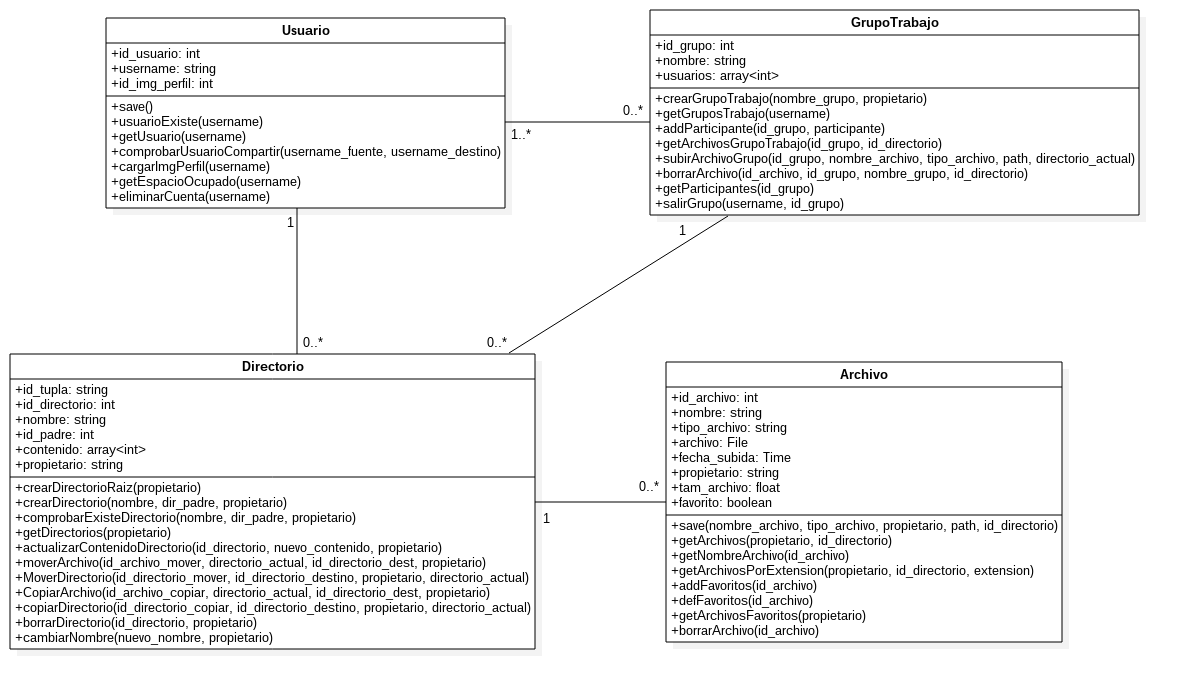
\includegraphics[width=1\textwidth]{imagenes/diagramasDeClases}
	\caption{Diagrama de clases del diseño.}
	\label{fig:diagramasDeClases}
\end{figure}


\chapter{Diseño}

En este apartado se comentarán los aspectos más importantes para el desarrollo de la aplicación. Para estudiar este apartado vamos a dividir el contenido en dos grupos: servidor (backend) y cliente (frontend).

\section{Backend}
El \textbf{backend} se encarga de recibir los datos desde el frontend y procesar dichos datos. \\

\subsection{Patrón Modelo-Vista-Controlador (MVC)}
Para el desarrollo de la aplicación se plantea el uso del patrón de arquitectura de software MVC, el cual se basa en separar los datos de la lógica de la aplicación y su interfaz. Ésto facilita el desarrollo y el posterior mantenimiento de la aplicación.
\begin{itemize}
	\item \textbf{Modelo} (Model): \textbf{información} con la que trabaja el sistema. Se encarga de gestionar los accesos a dicha información, tanto consultas como actualizaciones. Se corresponde con la base de datos.
	\item \textbf{Vista} (View): se refiere a los datos que se van a mostrar y como mostrarlos. La vista será el \textbf{frontend} de nuestra aplicación.
	\item \textbf{Controlador} (Controller): responde a \textbf{eventos} (generalmente los proporcionará el usuario) y llama al modelo cuando se realiza alguna solicitud sobre la información. También podrá enviar solicitudes a la vista si se solicita un cambio en la forma que mostrar la información. \\
\end{itemize}

\begin{figure}[H]
	\centering
	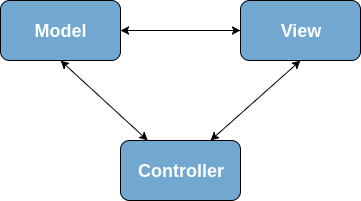
\includegraphics[width=0.7\textwidth]{imagenes/img_mvc}
	\caption{Diagrama Model-View-Controller.}
	\label{fig:img_mvc}
\end{figure}

\subsection{Django}
La decisión de usar el framework \textbf{Django} viene dada por su uso de la arquitectura MVC y su disponibilidad para trabajar con Python. Debido a que el controlador es manejado por el mismo framework y la parte más importante se produce en los modelos, las plantillas y las vistas, Django es conocido como un Framework MTV (Model- View - Template) \cite{cita_mvt}.
\begin{itemize}
	\item \textbf{Modelo} (Model): \textbf{información} con la que trabaja el sistema. Se encarga de gestionar los accesos a dicha información, tanto consultas como actualizaciones. Se corresponde con la base de datos.
	\item \textbf{Vista} (View): esta capa contiene la \textbf{lógica} que accede al modelo y la delega a la plantilla apropiada: actúa como puente entre el modelos y las plantillas.
	\item \textbf{Plantilla} (Template): se relaciona con la \textbf{presentación} de la información: como algunas cosas son mostradas sobre una página web u otro tipo de documento. \\
\end{itemize}

\begin{figure}[H]
	\centering
	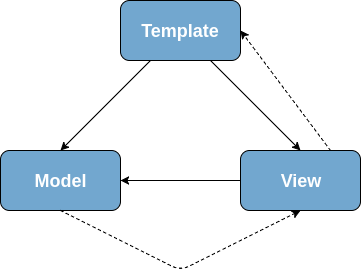
\includegraphics[width=0.7\textwidth]{imagenes/img_mvt}
	\caption{Diagrama Model-View-Template.}
	\label{fig:img_mvt}
\end{figure}

Django nos permite crear sitios web complejos ofreciendo diversos componentes que podemos usar para el desarrollo de nuestra aplicación.

\subsection{Sistema gestor de base de datos}
El sistema gestor de base de datos es el encargado de proporcionar la capa de acceso a la información de la base de datos. Haciendo uso del ORM de Django, utilizaremos un conector para la base de datos \textbf{MongoDB}.

\section{Frontend}
El \textbf{frontend} se refiere a la parte del sistema que se encarga de interactuar con los usuarios y mandar las peticiones al backend. Para interactuar con los usuarios hacemos uso de tecnologías web como \textbf{HTML}, \textbf{CSS} y \textbf{Javascript}. Este sistema trabaja todo el tiempo recibiendo peticiones de usuarios, por lo tanto usando las tecnologías mencionadas y añadiendo otras, como \textbf{jQuery}, haremos de nuestra interfaz un entorno intuitivo para los usuarios. \\

\subsection{jQuery}
\textbf{jQuery} es una librería de Javascript la cual ofrece la posibilidad de manipular los documentos HTML y manejar eventos, dotando a la web de una mayor dinamicidad. Es compatible con la mayoría de los navegadores actuales, tanto en pc como en dispositivos móviles. \\

\subsection{AJAX}
Por otro lado \textbf{AJAX} nos brinda la oportunidad de cargar datos desde el backend sin la necesidad de recargar toda la página del navegador. \\

\subsection{Twitter Bootstrap}
Otra tecnología usada de cara a la interacción con los usuarios de nuestra aplicación es la que nos aporta \textbf{Twitter Bootstrap}. Twitter Bootstrap es un framework CSS que nos facilita la tarea del diseño de la aplicación. Con esta tecnología podremos crear diseños muy elegantes y limpios, además de dotar a la aplicación web de un diseño adaptativo (responsive design) y así poder disfrutar de nuestra aplicación sin problemas en cualquier dispositivo y tamaño de pantalla. \\

\chapter{Implementación}

Tras haber visto la parte del diseño toca trabajar la implementación. En este apartado profundizaremos sobre el entorno de trabajo usado y la estructura de la aplicación.

\section{Entorno de trabajo}
Django nos da la posibilidad de trabajar con un "entorno virtual". Estos entornos son creados con el objetivo de aislar recursos, como son las librerías y el entorno de ejecución, del sistema principal o de otros entornos virtuales. Esto quiere decir que podemos tinstalar distintas versiones de una librería sin que se provoquen conflictos. \\
Para usar el entorno de trabajo hacemos uso de la herramienta \textbf{virtualenv}. Los comandos para crear un entorno y activarlo son los siguientes:

\begin{itemize}
	\item \textbf{Instalar virtualenv:} sudo pip install virtualenv
	\item \textbf{Crear entorno de trabajo:} virtualenv drawercloud\_env
	\item \textbf{Activar el entorno de trabajo:} source drawercloud\_env/bin/activate
\end{itemize}

Como podemos ver, para la instalación de virtualenv se ha usado \textbf{pip}. pip es la herramienta recomendada para instalar y administrar los paquetes de python. Los comandos que se usarán con más frecuencia son los que proceden:

\begin{itemize}
	\item \textbf{Instalar un paquete:} pip install <nombre\_paquete>
	\item \textbf{Desinstalar un paquete:} pip uninstall <nombre\_paquete>
	\item \textbf{Actualizar un paquete:} pip install <nombre\_paquete> --upgrade
	\item \textbf{Listar los paquetes instalados:} pip freeze
\end{itemize}

\textbf{Importante:} Todos los comandos se deberán usar con el entorno de trabajo activado.

\section{Estructura del proyecto}
A continuación se mostrarán las partes en las que se compone la estructura del proyecto. \\

\subsection{Fichero de configuración settings.py}
El fichero \textbf{settings.py} es el encargado de controlar la configuración del proyecto en Django. A continuación mencionaremos las opciones más destacables de este fichero según este proyecto:

\begin{itemize}
	\item \textbf{DEBUG:} cuando la variable DEBUG se encuentre igualada a \textbf{True} querrá decir que el sistema se ejecuta en modo "depuración", el cual nos proporcia los detalles de un error cuando éste se produzca. Cuando la aplicación se ejecute en "producción", a la variable le asignaremos el valor \textbf{False} por motivos de seguridad.
	
	\item \textbf{SECRET\_KEY:} es la llave secreta de nuestro proyecto y sirve para encriptar la información dentro de la base de datos.
	
	\item \textbf{INSTALLED\_APPS:} es una lista en la que se indica las aplicaciones habilitadas para este proyecto. Por ejemplo, para usar el administrador de Django añadimos la sentencia \textbf{'django.contrib.admin'}.
	
	\item \textbf{MIDDLEWARE:} es un framework que se usa como enlace en el proceso de solicitud/respuesta.
	
	\item \textbf{STATICFILES\_DIRS}: se indica la ruta a la carpeta \textbf{static} de nuestro proyecto. Dicha carpeta es la que contiene archivos relacionados con el frontend, como pueden ser los archivos CSS o los archivos Javascript.
	
	\item \textbf{connect(database\_name)}: esta función se ocupa de conectar con la base de datos indicada en el parámetro database\_name. \textbf{connect} es una función de MongoDB, para usarla haremos las siguientes importaciones:
	\begin{itemize}
		\item from pymongo import MongoClient
		\item from mongoengine import connect				
	\end{itemize}
	
	\item \textbf{REGISTRATION\_OPEN}: esta variable se igualará a \textbf{True} para permitir el registro de usuarios.
	
	\item \textbf{LOGIN\_REDIRECT\_URL}: indicamos la ruta a la que debe redirigirnos la aplicación una vez se ha realizado el log in con éxito.
	
	\item \textbf{LOGIN\_URL}: con esta variable decimos al sistema donde debemos aparecer en caso de no haber realizado el log in, o bien si se intenta acceder a páginas que requieren haberse logueado previamente.
\end{itemize}

Para obtener más información acerca del fichero de configuración settings.py de Django podemos visitar el enlace de la cita \cite{cita_django_settings}.

\subsection{Fichero de configuración urls.py}
En este fichero se indican las \textbf{URLs} que se van a usar en la aplicación. Tendremos dos ficheros urls.py. El que ahora comentamos se encontrará en la misma carpeta que el fichero settings.py mientras que el otro se encontrará en la carpeta del proyecto, la cual contiene los archivos como views.py, la carpeta static o la carpeta templates. En este apartado nos referimos al archivo urls.py almacenado junto a settings.py. En éste indicaremos las rutas a la página de administración, la ruta al resto de urls del proyecto y la ruta necesaria para el registro de usarios mediante django-registration-redux: \\

\begin{lstlisting}[language=python]
	urlpatterns = [
		url(r'^admin/', admin.site.urls),
		url(r'^proyecto/', include('proyecto.urls')),
		url(r'^accounts/', include('registration.backends.simple.urls')),
	]
\end{lstlisting}

\subsection{Fichero views.py}
El archivo \textbf{views.py} contiene las funciones que recibirán peticiones web y responderán a dichas peticiones también con un resultado web. Las respuestas prodrán ser un código HTML, una imagen, reproducir una canción, etc. El propio archivo contiene cualquier lógica que sea necesaria para poder devolver una respuesta. A modo de ejemplo vemos una vista simple como es la página principal de la sección "Multimedia" de nuestra aplicación. \\

\begin{lstlisting}[language=python]
	@login_required(login_url='/accounts/login/') #Requiere estar logueado para usar la funcion
	def multimedia(request):
		return render(request, 'multimedia.html', {'pagina_actual':'Multimedia'}) #Renderiza el fichero HTML multimedia.html
\end{lstlisting}

\subsection{Fichero models.py}
Recordamos que estamos usando una base de datos MongoDB. MongoDB es una base de datos orientada a documentos. Esto quiere decir que los datos no se guardan en registros, sino que se guardan en los denominados documentos. Éstos se almacenan en BSON, que nos es más que una representación binaria de JSON. \\

El fichero encargado para la gestión de documentos es el fichero \textbf{models.py}. En dicho fichero detallamos la estructura de los documentos que vayamos a crear. Por ejemplo, para el documento \textbf{Archivo} (usado para almacenar los archivos que se suban a drawercloud) tenemos la siguiente disposición: \\

\begin{lstlisting}[language=python]
	class Archivo(Document):
		id_archivo = DecimalField()
		nombre = StringField()
		tipo_archivo = StringField()
		archivo = FileField()
		fecha_subida = StringField()
		propietario = StringField()
		tam_archivo = DecimalField()
		favorito = BooleanField()
\end{lstlisting}


\subsection{Fichero forms.py}
En el archivo \textbf{forms.py} escribiremos toda la funcionalidad necesaria para gestionar los documentos de la base de datos. Las acciones tales como crear un usuario, almacenar un archivo, añadir un usuario a un grupo de trabajo... vendrán descritas en este fichero. Por ejemplo, la función para guardar un nuevo usuario quedaría de la siguiente manera: \\

\begin{lstlisting}[language=python]
	def save(self, _username):
		u = Usuario()
		
		u.username = _username
		u.id_username = Usuario.objects.count() + 1
		u.img_perfil = -1
		
		u.save()
		
		return u
\end{lstlisting}

\subsection{Fichero urls.py}
Nos encontramos aquí con el otro fichero \textbf{urls.py}. Dicho fichero contiene todas las urls de todas las funciones que se encuentran en el fichero views.py. Por ejemplo, para la función que se ocupa de descargar un archivo tendremos algo tal que así: \\

\begin{lstlisting}[language=python]
	url(r'^descargarArchivo/$', views.descargarArchivo, name='descargarArchivo'),
\end{lstlisting}

Analizando la sentencia, tenemos que el primer argumento es la url que tendrá en la web. El segundo argumento indica el nombre de la función en el fichero views.py. Por último, el tercer argumento indica el nombre con el cual nos podremos referir a la función cuando queramos invocarla, por ejemplo, desde un fichero HTML o Javascript. \\

\subsection{Directorio templates}
Este directorio contiene todos los archivos \textbf{HTML} que forman la vista de la aplicación. \\ 

\subsection{Directorio static}
Este directorio contiene todos los archivos \textbf{CSS, Javascript, imágenes, ...} que complementan a los archivos HTML almacenados en el directorio templates y que juntos forman el frontend. \\ 
\chapter{Pruebas}

Se han realizado distintas pruebas para estudiar el comportamiendo de la aplicación web (dichas pruebas se realizaron con la última versión de la aplicación). Para realizar las pruebas se ha usado la ayuda de un grupo de personas, las cuales han estado interactuando con la aplicación durante 10 minutos. Los resultados han sido los siguientes:

\section{Resultados de las pruebas con usuarios}
\chapter{Conclusiones y trabajos futuros}

\section{Conclusiones}
Tras la finalización del proyecto se ha obtenido un prototipo funcional de la aplicación web, que cumple con casi todas las expectativas y los objetivos marcados desde el principio, además de una completa memoria del proyecto. \\
 
Gracias a las pruebas realizadas con usuarios podemos determinar que...... \\

En definitiva tenemos que \textbf{drawercloud} cumple con los requisitos para efectuar su función principal de alojar archivos en la nube, a excepción del espacio disponible de almacenamiento actual que es insuficiente para una aplicación de estas características. Esto se debe a que el espacio que nos ofrece Amazon es solamente de 2GB, debiéndose esto a que se trata de la versión gratuita. No obstante esto tendría solución comprando más espacio de almacenamiento y ofreciendo a los clientes distintas versiones, las cuales serían de pago para grandes cantidades de espacio y una gratuita que ofrecería menos capacidad. \\

\subsection{Conocimientos adquiridos}
Gracias al análisis y al desarrollo de este proyecto se han adquirido conocimientos en diversos ámbitos del desarrollo de software, en su mayoría en el sector web. Entre los conocimientos adquiridos podemos nombrar: 

\begin{itemize}
	\item Se ha profundizado mucho en el uso del lenguaje de programación \textbf{Python}, así como en el framework para desarrollo web \textbf{Django}, proporcionando así conocimientos de la arquitectura \textbf{MVC}.
	\item Técnicas para el desarrollo de interfaces web gracias a tecnologías como \textbf{Bootstrap} \textbf{jQuery} y \textbf{AJAX}.
	\item Realizar \textbf{pruebas con usuarios} para permitir encontrar errores o descubrir funcionalidades que podamos aplicar para hacer una aplicación más completa y competitiva.
	\item Aprender a realizar un correcto \textbf{desarrollo de la documentación}.
\end{itemize}

\section{Trabajos futuros}
drawercloud ofrece la funcionalidad necesaria para ser una herramienta de almacenamiento de archivos en la nube, pero para ello aún se deben pulir algunos aspectos y convertirla en un serio competidor. Para ello se deberían tener en cuenta algunas evoluciones en el software como las siguientes:

\begin{itemize}
	\item Comprar espacio de almacenamiento.Esta opción sería la maś importante ya que no disponemos de espacio suficiente para competir con otras aplicaciones de este tipo.
	\item Permitir subir \textbf{varios archivos} a la vez.
	\item Incluir las opciones de \textbf{arrastrar para mover} y \textbf{seleccionar} varios archivos.
	\item Añadir un \textbf{visor} de imágenes y \textbf{reproductores} de audio y vídeo más estéticos y con mayor funcionalidad.
	\item Perfeccionar aspectos de \textbf{rendimiento}	a la hora de subir archivos.
	\item Crear una versón de la aplicación para \textbf{móvil} y para \textbf{escritorio}.
\end{itemize}

\chapter{Manual de usuario}

\section{Acceso a la aplicación}
La primera página que se carga de nuestra aplicación web es la que se refiere al login. En la imagen \ref{fig:login} podemos consultar el aspecto de dicha página. Observamos dos entradas de texto, una para insertar el nombre de usuario y otra para la contraseña. \\

Para usuarios que no estén registrados se presenta la opción de \textbf{Crear una nueva cuenta}, en la cual debemos rellenar los datos requeridos: nombre de usuario, dirección de correo electrónico, contraseña y confirmar contraseña. En la imagem \ref{fig:registro}

\begin{figure}[H]
	\centering
	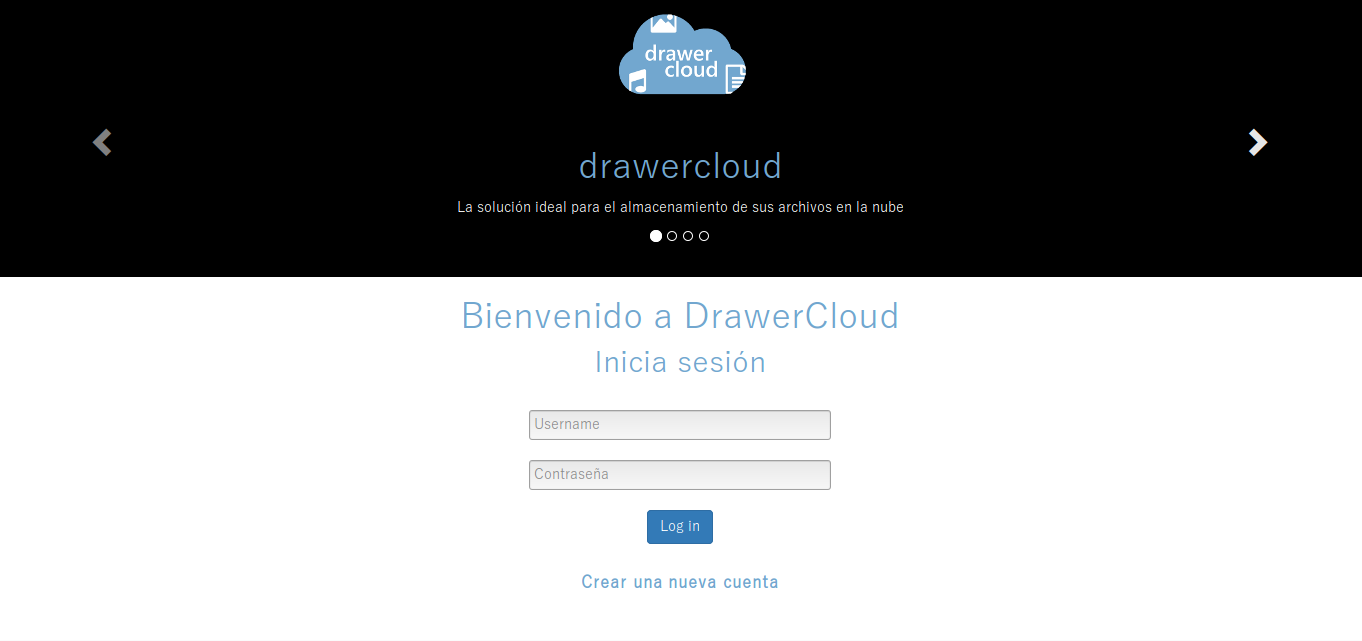
\includegraphics[width=1\textwidth]{imagenes/login}
	\caption{Acceso a la aplicación. Página de login}
	\label{fig:login}
\end{figure}

\begin{figure}[H]
	\centering
	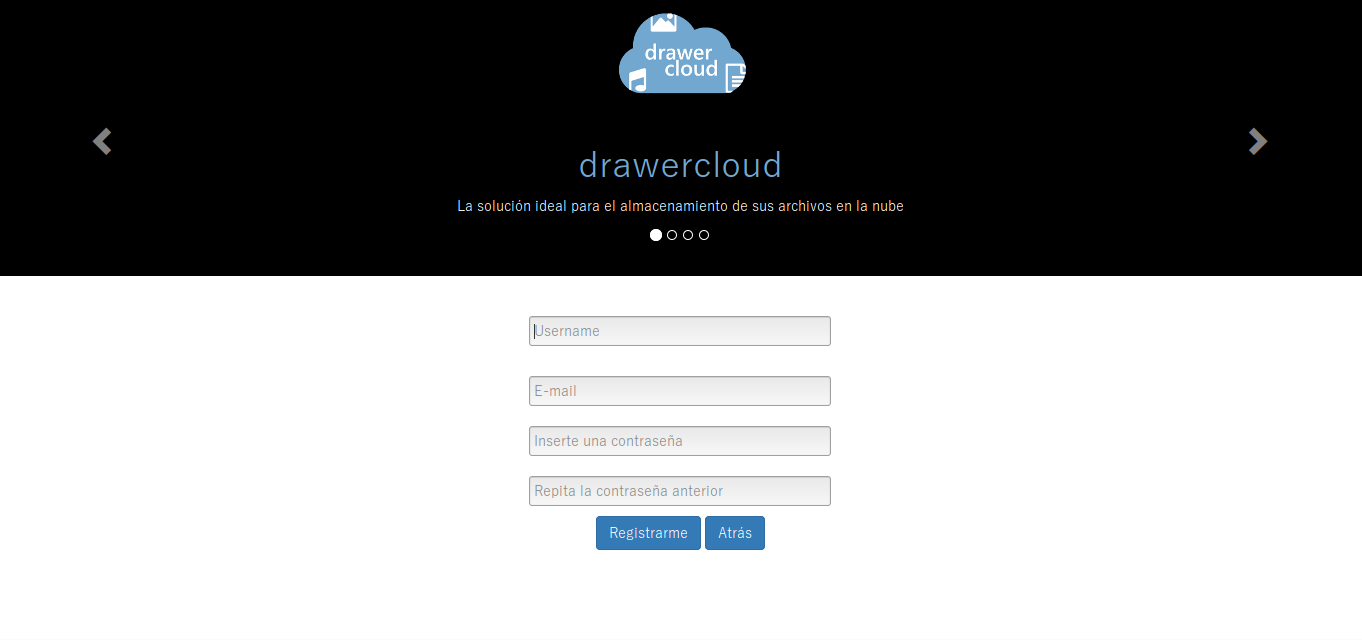
\includegraphics[width=1\textwidth]{imagenes/registro}
	\caption{Acceso a la aplicación. Página de registro}
	\label{fig:registro}
\end{figure}

\section{Página principal - Documentos}
La página principal es la sección \textbf{Documentos} \ref{fig:documentos}. En esta página nos encontraremos con una estructura de directorios y archivos. La vista en que se muestran los directorios y archivos se podrá cambiar haciendo uso de los botones de la imagen \ref{fig:bts_cambiar_vista}, estando disponibles dos tipos de vista: lista \ref{fig:documentos} o iconos \ref{fig:documentos_iconos}.


\begin{figure}[H]
	\centering
	\begin{subfigure}{0.4\textwidth}
		\centering
		
\includegraphics[width=.4\linewidth]{imagenes/bt_cambiar_vista_iconos}
		\caption{Cambiar a la vista \textbf{iconos}}
		\label{fig:bt_cambiar_vista_iconos}
	\end{subfigure}%
	\begin{subfigure}{0.4\textwidth}
		\centering
		
\includegraphics[width=.4\linewidth]{imagenes/bt_cambiar_vista_lista}
		\caption{Cambiar a la vista \textbf{lista}}
		\label{fig:bt_cambiar_vista_lista}
	\end{subfigure}
	\caption{Botones disponibles para cambiar la vista}
	\label{fig:bts_cambiar_vista}
\end{figure}

\begin{figure}[H]
	\centering
	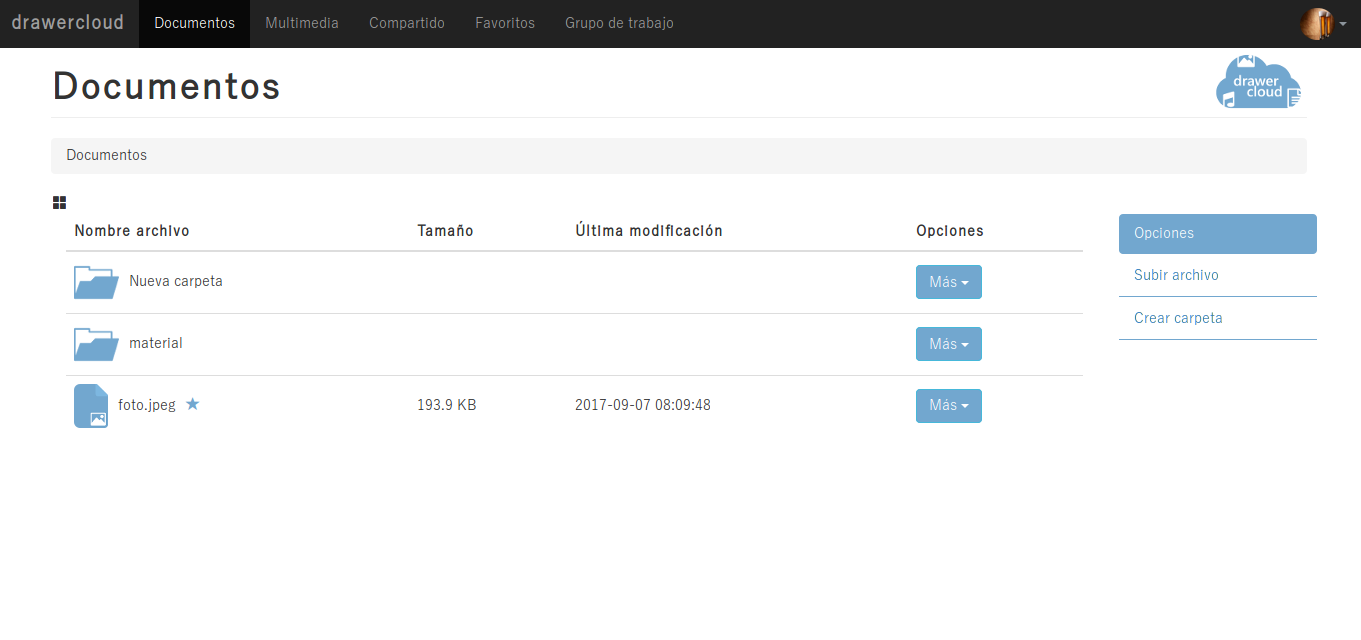
\includegraphics[width=1\textwidth]{imagenes/documentos}
	\caption{Documentos. Aspecto de la página principal}
	\label{fig:documentos}
\end{figure}

\begin{figure}[H]
	\centering
	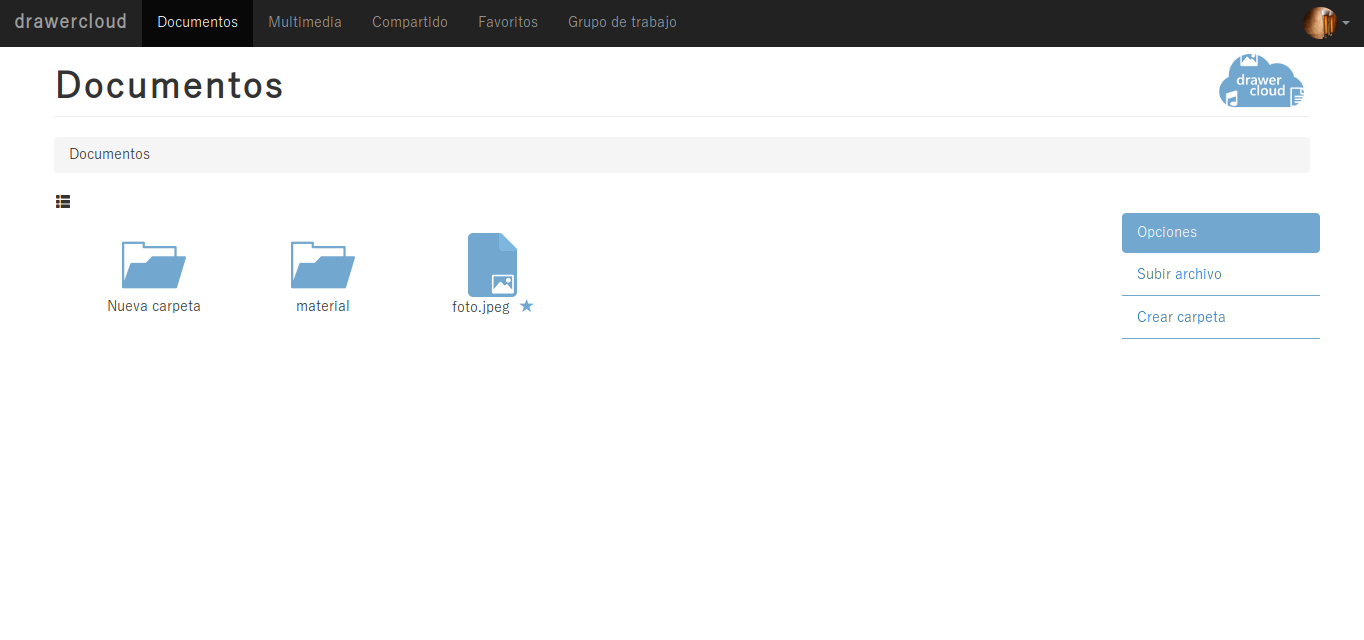
\includegraphics[width=1\textwidth]{imagenes/documentos_iconos}
	\caption{Documentos. Aspecto de la página principal}
	\label{fig:documentos_iconos}
\end{figure}

En \textbf{Documentos} vamos a poder almacenar los archivos que deseemos, podiendo organizar tales archivos en directorios. Para \textbf{crear directorios} o \textbf{subir archivos} hacemos uso de las opciones que aparecen a la derecha de la página documentos \ref{fig:opciones_documentos}.

\begin{figure}[H]
	\centering
	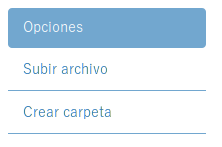
\includegraphics[width=0.4\textwidth]{imagenes/opciones_documentos}
	\caption{Documentos. Opciones de la página Documentos}
	\label{fig:opciones_documentos}
\end{figure}

Los archivos y directorios disponen de \textbf{funcionalidades} propias, como la posibilidad de descargar un archivo, copiar un directorio, etc. Para acceder a estas opciones podemos elegir entre hacer \textbf{click derecho} sobre los directorios/archivos o seleccionar el botón \textbf{Más} disponible para la vista lista.

\subsection{Opciones para archivos}
\begin{itemize}
	\item \textbf{Descargar:}
	\item \textbf{Compartir:}
	\item \textbf{Cambiar nombre:}
	\item \textbf{Copiar en:}
	\item \textbf{Mover a:}
	\item \textbf{Añadir a favoritos:}
	\item \textbf{Eliminar:}
\end{itemize} 

\subsection{Opciones para directorios}
\begin{itemize}
	\item \textbf{Cambiar nombre:}
	\item \textbf{Copiar en:}
	\item \textbf{Mover a:}
	\item \textbf{Eliminar:}
\end{itemize} 
%
%%\chapter{Conclusiones y Trabajos Futuros}
%
%
%%\nocite{*}
%\bibliography{bibliografia/bibliografia}\addcontentsline{toc}{chapter}{Bibliografía}
%\bibliographystyle{miunsrturl}
%
%\appendix
%\input{apendices/manual_usuario/manual_usuario}
%%\input{apendices/paper/paper}
%\input{glosario/entradas_glosario}
% \addcontentsline{toc}{chapter}{Glosario}
% \printglossary
\chapter*{}
\thispagestyle{empty}


\newpage
\bibliography{citas} %archivo citas.bib que contiene las entradas 
\bibliographystyle{ieeetr} % hay varias formas de citar
\end{document}
